\begin{thwbr}
\chapter{ไฟล์}
\begin{flushright}
{\it\latintext ``Everything in the Unix system is a file.''}\\
{\bf\latintext  Brian W. Kernighan, Rob Pike \cite{upe}}
\end{flushright}

ในหนังสือ The Unix Programming Environment \cite{upe} ซึ่งจัดเป็นหนังสือต้องมีเล่มหนึ่งสำหรับผู้ใช้ยูนิกซ์กล่าวไว้ว่า ``ทุกอย่างในยูนิกซ์คือไฟล์''. ประโยคยังเป็นความจริงสำหรับระบบปฏิบัติการลินุกซ์ด้วย. ในการใช้ลินุกซ์ในแต่ละวัน, การทำงานกับไฟล์เป็นสิ่งที่หลีกเลี่ยงไม่ได้ ตั้งแต่การสร้างไฟล์, แก้ไขไฟล์ ฯลฯ. ดังนั้นจึงมีความจำเป็นที่จะต้องเรียนรู้เกี่ยวกับไฟล์ในลินุกซ์เป็นอย่างดีในบทนี้.


\section{พาร์ทิชัน, และระบบไฟล์}
ปรกติแล้ว, ไฟล์ที่ใช้ในระบบปฏิบัติการลินุกซ์จะอยู่ในหน่วยความถาวรเช่นฮาร์ดดิสก์. และก่อนที่จะสร้างไฟล์ในฮาร์ดดิสก์ได้นั้นต้องสร้างพาร์ทิชันและสร้างระบบไฟล์ให้กับพาร์ทิชันนั้นก่อนจึงจะสามารถกระทำการต่างๆกับไฟล์ได้.

\subsection{พาร์ทิชัน}
\emph{พาร์ทิชัน (partition)} คือหน่วยย่อยของฮาร์ดดิกส์, หรือฮาร์ดดิสก์ย่อยแบบ logical ที่แบ่งมาจากฮาร์ดดิกส์ที่มีอยู่จริง. พาร์ทิชันยังแบ่งได้เป็นสองประเภทคือ\emph{พาร์ทิชันหลัก (primary partition)} และ\emph{พาร์ทิชันเสริม (extended partition)}. เราสามารถแบ่งพาร์ทิชันหลักได้มากที่สุด 4 ส่วน. ถ้าต้องการแบ่งพาร์ทิชันมากกว่านั้นต้องให้พาร์ทิชันหลักหนึ่งในสี่นั้นเป็นพาร์ทิชันเสริมตามที่แสดงในรูปที่ \ref{fig:partition}. ในพาร์ทิชันสามารถสร้างพาร์ทิชันที่เรียกว่าพาร์ทิชัน logical ต่อไปได้อีกเรื่อยๆ.


\begin{figure}[!htbp]
\plfigure{1.0}{partition.eps}{พาร์ทิชันหลักและพาร์ทิชันเสริม.}{partition}
\end{figure}

ข้อมูลตำแหน่งของพาร์ทิชันเหล่านี้จะเก็บอยู่ในส่วนที่เรียกว่า \emph{partition table} และโปรแกรมที่ทำหน้าที่จัดการข้อมูลพาร์ทิชันของฮาร์ดดิสก์ได้แก่โปรแกรม \cmd{fdisk}.\cindex{fdisk}\refcmd{fdisk} โปรแกรมนี้จะใช้โดยผู้ดูแลระบบหรือ root เพื่อจัดการแบ่งพาร์ทิชันและกำหนดประเภทของพาร์ทิชัน. 

\begin{MyExample}[ใช้ \cmd{fdisk} แสดง partition table.]
\begin{MyEx}
# \cin{fdisk /dev/hdb} \mycomment{ฮาร์ดดิสก์แบบ EIDE ตัวที่สอง. ตัวแรกจะมีชื่อเป็น hda}
                                                                                
The number of cylinders for this disk is set to 38166.
There is nothing wrong with that, but this is larger than 1024,
and could in certain setups cause problems with:
1) software that runs at boot time (e.g., old versions of LILO)
2) booting and partitioning software from other OSs
   (e.g., DOS FDISK, OS/2 FDISK)
                                                                                
Command (m for help): \cin{p}
                                                                                
Disk /dev/hdb: 40.0 GB, 40020664320 bytes
64 heads, 32 sectors/track, 38166 cylinders
Units = cylinders of 2048 * 512 = 1048576 bytes
                                                                                
   Device Boot      Start         End      Blocks   Id  System
/dev/hdb1               1       19074    19531760   83  Linux
/dev/hdb2           19075       37672    19044352   83  Linux
/dev/hdb3           37673       38166      505856   82  Linux swap
                                                                                
Command (m for help): \cin{q}
                                                                                
# \cursorprompt
\end{MyEx}
\end{MyExample}

สำหรับระบบปฏิบัติการลินุกซ์แล้ว, ควรจะแบ่งพาร์ทิชันอย่างน้อย 2 ส่วนขึ้นไป. ส่วนแรกใช้สำหรับเป็นพื้นที่ที่จะสร้างระบบไฟล์เพื่อเก็บข้อมูลที่จำเป็นต่อไป. ส่วนพาร์ทิชันทีเหลือใช้เป็นพื้นที่สำหรับ virtual memory\gindex{virutual memory}\myvocab{v}{virtual memory}{} ซึ่งมักจะเรียกกันว่า \emph{swap partition}\gindex{swap partition}. swap partition มีไว้สำหรับให้เคอร์เนลเก็บข้อมูลบางส่วนที่อยู่ในหน่วยความจำชั่วคราว (memory) ลงในฮาร์ดดิสก์ได้. และเรียกข้อมูลส่วนนั้นที่อยู่ในฮาร์ดดิสก์กลับมาในหน่วยความจำใหม่เมื่อต้องการ. วิธีการนี้ทำให้จำนวนหน่วยความจำโดยรวมไม่ขาดแคลน, และในบางกรณีสามารถช่วยให้ประสิทธิภาพการทำงานของโปรแกรมบางอย่างดีขึ้นด้วย. \mymemo{ผู้ใช้สามารถระบบที่ไม่มี swap ก็ได้แต่ไม่แนะนำ. พื้นที่ที่เป็น swap นี้ไม่จำเป็นต้องเป็นพาร์ทิชันแต่อาจจะเป็นไฟล์ก็ได้. swap ที่เป็นไฟล์นั้นมักจะสร้างเมื่อต้องการเพิ่มจำนวน swap ภายหลังที่สร้างพาร์ทิชันไปเรียบร้อยแล้ว.}


\subsection{ระบบไฟล์}
การสร้างพาร์ทิชันเป็นเพียงแค่การแบ่งฮาร์ดดิสก์ให้มีจำนวนและขนาดตามที่ต้องการ. พาร์ทิชันที่สร้างขึ้นมานั้นต้องผ่านการสร้าง\emph{ระบบไฟล์ (file system)} ก่อนจึงจะใช้งาน, อ่านเขียนไฟล์ได้. การสร้างระบบไฟล์ในพาร์ทิชันเป็นการสร้างข้อมูลพื้นฐานเพื่อที่จะเก็บข้อมูลเป็นไฟล์, จัดโครงไดเรกทอรีต่อไป. การจัดเก็บไฟล์และไดเรกทอรีในระบบปฏิบัติการลินุกซ์และยูนิกซ์จะมีโครงสร้างเป็นแผนภาพต้นไม้ตามรูปที่ \ref{fig:directory_struct}.

\begin{figure}[!htb]
\plfigure{.7}{directory_struct.eps}{โครงสร้างไฟล์และไดเรกทอรี}{directory_struct}
\end{figure}

ระบบไฟล์ที่ออกแบบมาสำหรับลินุกซ์เพื่อสร้างโครงสร้างไฟล์และไดเรกทอรีมีหลายประเภทเช่น ext2 (Second Extended Filesystem), ext3, xfs, Reiserfs ฯลฯ. ระบบไฟล์เหล่านี้จะเก็บข้อมูลเกี่ยวกับตำแหน่งของไฟล์ต่างๆและข้อมูลที่เกี่ยวข้องอื่นๆเช่น ข้อมูลเกี่ยวกับเจ้าของไฟล์, สิทธิ์ในการใช้ไฟล์, เวลาบันทึกไฟล์ เป็นต้น. 


การสร้างระบบไฟล์ให้กับพาร์ทิชันที่แบ่งไว้แล้วจะใช้คำสั่ง \cmd{mkfs} ซึ่ง root มักจะเป็นผู้ใช้คำสั่งนี้สร้างระบบไฟล์.\cindex{mkfs}\refcmd{mkfs}

\begin{MyExample}[การสร้างระบบไฟล์.]
\begin{MyEx}
# \cin{mkfs -t ext2 /dev/fd0}
\end{MyEx}
\end{MyExample}

ในความเป็นจริงแล้วคำสั่ง \cmd{mkfs} เป็นเพียง front-end\myvocab{f}{front-end}{โปรแกรมที่เรียกใช้โปรแกรมเฉพาะต่ออีกทีหนึ่ง. เช่นโปรแกรม \cmd{mkfs} เรียกใช้โปรแกรม \cmd{mkfs.ext2} หรือ \cmd{mkfs.xfs} อีกทอดหนึ่งแล้วแต่ตัวเลือกที่ใช้กับ \cmd{mkfs}. โปรแกรม front-end เหล่านี้เป็นเพียงอินเทอร์เฟส, ไม่ได้เป็นตัวที่ทำงานหลักเอง.} ของโปรแกรมที่สร้างระบบไฟล์อื่นๆเช่น \cmd{mkfs.ext2}, \cmd{mkfs.xfs} ฯลฯ. ดังนั้นเราอาจจะเรียกใช้โปรแกรม \cmd{mkfs.ext2} โดยตรงก็ได้.

นอกจากระบบไฟล์ที่ออกแบบมาสำหรับลินุกซ์แล้ว, เรายังสามารถสร้างหรือใช้ระบบไฟล์อื่นๆเช่นระบบไฟล์สำหรับ DOS, vfat (วินโดวส์), ntfs (วินโดวส์) ฯลฯ และนำมาใช้กับลินุกซ์ได้ด้วย. ปรกติเราจะสร้างระบบไฟล์เหล่านี้ให้กับฮาร์ดดิสก์พกพา, USB flash memory, ฟล็อปปี้ดิสก์ เพื่อที่จะได้ใช้กับเครื่องคอมพิวเตอร์วินโดวส์ได้ด้วย. 

\subsection{mount และ unmount}

\begin{figure}[!htb]
\plfigure{.7}{mount.eps}{mount พาร์ทิชันเข้าในโครงสร้างไฟล์.}{mount}
\end{figure}

ขั้นตอนต่อไปเพื่อที่จะใช้พาร์ทิชันที่สร้างระบบไฟล์เรียบร้อยแล้วเก็บบันทึกไฟล์ได้แก่การ \emph{mount}\gindex{mount} ระบบไฟล์นั้นเข้าไปในโครงสร้างไฟล์และไดเรกทอรีที่แสดงในรูปที่ \ref{fig:directory_struct}. 

การ mount คือการนำระบบไฟล์ที่สร้างในพาร์ทิชัน (ดีไวซ์, ฮาร์ดดิสก์) ไปปะติดกับโครงสร้างไดเรกทอรีที่ในตำแหน่งที่ต้องการ. ตำแหน่งที่นำระบบไฟล์ไปปะติดนี้เรียกว่า\emph{จุด mount (mount point)} ซึ่งจะเป็นไดเรกทอรีที่สร้างเตรียมไว้\mymemo{จะเป็นไดเรกทอรีที่ว่างเปล่าหรือไม่ว่างเปล่าก็ได้.}. ตัวอย่างเช่นรูปที่ \ref{fig:mount}, ระบบไฟล์ที่สร้างไว้บนพาร์ทิชันที่ 1 จะปะติดกับไดเรกทอรี \cmd{/} (รูท). ไดเรกทอรี \cmd{/home} สร้างในพาร์ทิชันที่ 1 แต่หลังจากที่ mount ระบบไฟล์ที่สร้างไว้บนพาร์ทิชันที่ 2 ปะติดกับไดเรกทอรี \cmd{/home} แล้ว, ข้อมูลที่อยู่ใต้ไดเรกทอรี \cmd{/home} จะไปเก็บอยู่ในพาร์ทิชันที่ 2. การ mount ไม่จำเป็นต้อง mount กับพาร์ทิชันหรือฮาร์ดดิสก์เสมอไป, อาจจะ mount ระบบไฟล์ที่อยู่ในเครื่องคอมพิวเตอร์อื่นๆผ่านทางเน็ตเวิร์กก็ได้\mymemo{ระบบไฟล์ที่ใช้เน็ตเวิร์กเช่น smbfs (Samba filesystem), netfs (network filesystem) เป็นต้น.}. ตอนที่เครื่องเริ่มทำงานจะ mount ระบบไฟล์ต่างๆตามที่กำหนดไว้ในไฟล์ \cmd{/etc/fstab}.

\bigskip
คำสั่ง \cmd{mount}\refcmd{mount} เป็นคำสั่งที่ใช้ mount ระบบไฟล์เข้าไปในไดเรกทอรีหรือดูระบบไฟล์และไดเรกทอรีที่ mount อยู่.

\begin{MyExample}[คำสั่ง \cmd{mount} แสดงระบบไฟล์ที่ mount อยู่.]
\begin{MyEx}
$ \cin{mount}
/dev/hdb1 on / type ext3 (rw,noatime)
devfs on /dev type devfs (rw)
none on /proc type proc (rw)
none on /sys type sysfs (rw)
none on /dev/pts type devpts (rw)
/dev/hdb2 on /home type ext3 (rw,noatime)
none on /dev/shm type tmpfs (rw)
none on /proc/bus/usb type usbfs (rw)
/dev/hda2 on /mnt/usb type ntfs (rw,uid=1000)
/dev/cdrom on /mnt/cdrom type iso9660 (ro)
\end{MyEx}
\end{MyExample}%$

เนื่องจากการ mount เป็นการนำระบบไฟล์เข้าไปปะติดกับไดเรกทอรีที่ต้องการในโครงสร้างไฟล์และไดเรกทอรี, ดังนั้นจากมุมมองของผู้ใช้แล้วเราจึงมองโครงสร้างไฟล์และไดเรกทอรีได้เป็นหนึ่งเดียวคือในรูปที่ \ref{fig:directory_struct}, ไม่มีการบอกว่าไดเรกทอรีนี้เป็นของพาร์ทิชันนี้ชัดเจนเหมือนระบบปฏิบัติการวินโดวส์ที่ใช้ตัวอักษรภาษาอังกฤษกำกับพาร์ทิชัน.


คำสั่ง \cmd{mount} ที่ใช้ mount ระบบไฟล์ปะติดกับไดเรกทอรีต้องใช้ตัวเลือก \cmd{-t} (type) เพื่อระบุระบบไฟล์และมีชื่อไฟล์เป็นอาร์กิวเมนต์ดังต่อไปนี้.
\begin{MyExample}[การ mount ฟล็อปปี้ดิสก์.]
\begin{MyEx}
# \cin{mount -t ext2 /dev/fd0 /mnt/floppy -o ro}
\end{MyEx}
\end{MyExample}
จากตัวอย่างเป็นการ mount ฟล็อปปี้ปะติดกับไดเรกทอรี \cmd{/mnt/floppy}.\mymemo{ต้องสร้างไดเรกทอรีที่ต้องการ mount เตรียมไว้ก่อนเสมอ.} ตัวเลือก \cmd{-o} (option) เป็นการระบุรายละเอียดปลีกย่อยของการ mount. ในตัวอย่าง ``ro'' คือ read-only ให้อ่านได้อย่างเดียวเท่านั้น, ไม่สามารถเขียนได้. รายละเอียดปลีกย่อยนี้บางอย่างจะขึ้นกับระบบไฟล์ที่ใช้, ให้อ่านรายละเอียดเพิ่มเติมจาก \cmd{mount(8)}. หลังจากที่ mount เรียบร้อยแล้วผู้ใช้ก็สามารถอ่านไฟล์ที่อยู่ในฟล็อปปี้ได้จากไดเรกทอรี \cmd{/mnt/floppy}. 

\begin{table}[!htb]
\caption{ระบบไฟล์ที่ใช้ในลินุกซ์.}\label{tab:filesystem}
\medskip
\begin{tabular}{lp{.8\textwidth}}
\toprule
\multicolumn{1}{c}{ระบบไฟล์} & \multicolumn{1}{c}{คำอธิบาย}\\
\midrule
ext2 & เป็นระบบไฟล์มาตรฐานสำหรับลินุกซ์. เดิมเป็นระบบไฟล์ที่นิยมใช้ในลินุกซ์. แต่ในปัจจุบันเริ่มใช้ extended 3 ซึ่งเป็นระบบไฟล์ที่พัฒนาต่อจาก extended 2 อีกที.\\
ext3 & เป็นระบบไฟล์แบบ ext2 ที่มีคุณสมบัติ journal เพิ่มเติม.\\
fat, vfat & ระบบไฟล์ที่ใช้ใน DOS, วินโดวส์.\\
ntfs & ระบบไฟล์ที่ใช้ในวินโดวส์ 2000 หรือ XP.\\
iso9660 & เป็นระบบไฟล์ที่มักใช้กับแผ่นซีดี.\\
smbfs & ระบบไฟล์แบบเน็ตเวิร์ก, ใช้สำหรับ mount ไดเรกทอรีที่แชร์จากเครื่องวินโดวส์หรือเซิฟร์เวอร์ที่ใช้ samba.\\
nfs & ระบบไฟล์ Network File System. สำหรับใช้ไฟล์ผ่านเน็ตเวิร์กระหว่างเครื่องยูนิกซ์หรือลินุกซ์.\\
reiserfs, xfs, jfs & ระบบไฟล์สมัยใหม่ที่ออกแบบโดยคำนึงถึงประสิทธิภาพการทำงานด้านต่างๆเช่นความเร็ว, ขีดจำกัดของขนาดไฟล์, ระบบ journal เป็นต้น.\\
\bottomrule
\end{tabular}
\end{table}

\bigskip
unmount คือการเอาระบบไฟล์ออกจากไดเรกทอรีที่ mount อยู่. คำสั่งที่ใช้สำหรับ unmount ได้แก่ \cmd{umount}.\cindex{umount}\refcmd{umount}\mymemo{ใหระวังชื่อคำสั่งคือ \cmd{umount} ไม่ใช่ \cmd{unmount}} ตัวอย่างเช่น 
\begin{MyExample}[การ unmount.]
\begin{MyEx}
# \cin{umount /mnt/floppy}
\end{MyEx}
\end{MyExample}
จากมุมมองของระบบปฏิบัตการ, ถ้ามีข้อมูลที่ต้องเขียนลงระบบไฟล์นั้นแต่ข้อมูลนั้นยังอยู่ในหน่วยความจำชั่วคราว, ก็จะทำการเขียนลงระบบไฟล์นั้น. การกระทำนี้เรียกว่า \emph{sync} (synchronize) ข้อมูลเพื่อให้ข้อมูลถูกต้องก่อนจะเอาระบบไฟล์ออกจากโครงสร้างไดเรกทอรี. นอกจากจะ sync ข้อมูลแล้ว, เคอร์เนลยังตรวจสอบด้วยว่ามีไฟล์ใดบ้างที่ยังเปิดอยู่หรือมีโปรแกรมใช้ไฟล์ที่อยู่ในระบบไฟล์นั้นหรือไม่. ถ้ามีก็ไม่สามารถ unmount ได้และจะเกิด error ว่า ``device is busy''. ในกรณีนี้ต้องกำจัดโปรเซสที่เปิดไฟล์ใต้ไดเรกทอรีนั้นให้หมดก่อนจึงจะ unmount ได้.

\section{ไฟล์}
\emph{ไฟล์ (file)}\gindex{file}\gindex{ไฟล์} %
\mymemo{ในภาษาไทยอาจแปลคำว่า file เป็นแฟ้มข้อมูล.}%
คืออะไร? ไฟล์คือกลุ่มก้อนของข้อมูล. ข้อมูลนี้มีจุดเริ่มต้นและจุดจบ. ตั้งแต่จุดเริ่มต้นจนถึงจุดจบจะเป็นข้อมูลต่อเนื่องไปเรื่อยๆเป็น\emph{สายข้อมูล (data stream)}. สรุปแนวคิดของไฟล์สั้นได้ว่า, ไฟล์คือสายข้อมูล. สายข้อมูลนี้ไม่มีการแยกแยะประเภทของข้อมูลว่าจะเป็น\emph{ไบนารี (binary)} หรือ\emph{เท็กซ์ (text)}. ความแตกต่างของข้อมูลไบนารีและข้อมูลเท็กซ์เป็นเพียงความแตกต่างที่มนุษย์สังเกตุเห็น, คือเป็นข้อมูลอักขระที่มนุษย์อ่านได้หรืออ่านไม่ได้เท่านั้น. สำหรับคอมพิวเตอร์แล้ว, ข้อมูลคือค่าที่แสดงในหน่วยของ\emph{ไบต์ (byte)} %
\myvocab{b}{byte}{หน่วยของข้อมูล. จำนวนหนึ่งไบต์สามารถแสดงหรือเก็บค่าได้ตั้งแต่ 0 ถึง 255.}.%
จริงไม่มีการแยกแยะความแตกต่างระหว่างข้อมูลไบนารีกับข้อมูลเท็กซ์.

\subsection{ชื่อไฟล์}
ไฟล์ต้องมีชื่อและจำนวนอักขระที่สามารถใช้เป็นชื่อไฟล์มีขนาดไม่เกิน 255 ตัวอักษร\mymemo{ขีดจำกัดนี้ดูได้จาก \cmd{limit.h} ที่อยู่ในรหัสต้นฉบับของเคอร์เนล.}. ชื่อไฟล์สามารถใช้อักษรหรือเครื่องหมายได้แต่ในทางปฏิบัติควรจะหลีกเลี่ยงเครื่องหมายที่มีความหมายพิเศษสำหรับเชลล์เช่น ช่องไฟ, วงเล็บ \cmd{()} เป็นต้น. เนื่องจากช่องไฟเป็นตัวแบ่งอาร์กิวเมนต์ในเชลล์จึงไม่ควรใช้ช่องไฟในชื่อไฟล์ถ้าไม่มีความจำเป็นจริงๆ. โดยทั่วไปมักจะใช้เครื่องหมาย underscore (\cmd{\_}) แทนช่องไฟ. ตัวอย่างเช่นแทนที่จะใช้ชื่อไฟล์ ``\cmd{important file}'' ก็ใช้ ``\cmd{important\_file}'' แทน. นอกจากนี้ลินุกซ์ยังแยกแยะความแตกต่างระหว่างอักษรตัวใหญ่ (capital letter) และอักษรตัวเล็ก (small letter) ด้วย.

สำหรับระบบที่ปรับแต่งให้ใช้\emph{ภาษานานาชาติ (internationalization, i18n)}\myvocab{i}{internationalization}{ความสามารถที่โปรแกรมสามารถปรับตัวให้เข้ากับสภาพแวดล้อมภาษาและวัฒนธรรมที่ผู้ใช้กำหนด. ตัวอย่างเช่นโปรแกรมสามารถแสดงผลนอกเหนือจากภาษาอังกฤษได้ถ้าสภาพแวดล้อมของผู้ใช้ไม่ใช่ภาษาอังกฤษ. Internationalization มีคำย่อว่า i18n โดยตัวเลข 18 คือจำนวนอักษรระหว่างอักษร i และ n.} ได้ก็สามารถใช้ภาษาอื่นนอกจากภาษาอังกฤษเป็นชื่อไฟล์ได้ด้วย. แต่อย่างไรก็ตามหากมีการก็อปปี้ไฟล์นั้นข้ามระบบ, หรือใช้กับคอมพิวเตอร์อื่นๆก็ควรจะใช้ภาษาอังกฤษเป็นชื่อไฟล์เพื่อหลีกเลี่ยงปัญหาที่เกิดขึ้นจากเครื่องคอมพิวเตอร์อื่นที่อาจจะไม่สนับสนุนการใช้ภาษานานาชาติ.

\subsubsection{ส่วนขยายชื่อไฟล์}
เนื่องจากไฟล์คือสายข้อมูล, และชื่อไฟล์จะใช้ตัวอักษรหรือเครื่องหมายอะไรก็ได้, หมายความว่า\emph{ส่วนขยายชื่อไฟล์ (filename extension)} %
\gindex{ส่วนขยายชื่อไฟล์}\gindex{filename extension}%
เช่น \cmd{.txt}, \cmd{.zip} ฯลฯ เป็นเพียงแค่ส่วนหนึ่งของชื่อไฟล์และไม่มีความหมายพิเศษสำหรับโปรแกรมที่ใช้ไฟล์นั้น. กล่าวคือไม่ว่าไฟล์จะชื่อ \cmd{file.txt} หรือ \cmd{file} อย่างเดียว, ถ้าไม่เปิดดูเนื้อหาของไฟล์ข้างในก็จะไม่รู้ว่าไฟล์นั้นเป็นไฟล์แบบไหน. 

ในลินุกซ์จะมีคำสั่ง \cmd{file} %
\cindex{file}%
\refcmd{file}%
เพื่อใช้ตรวจสอบประเภทของไฟล์. ตัวอย่างเช่น,
\begin{MyExample}[การใช้ \cmd{file} ตรวจสอบประเภทของไฟล์.]\label{ex:filetype}
\begin{MyEx}
$ \cin{file /etc/passwd /bin/bash}
/etc/passwd: ASCII text
/bin/bash:   ELF 32-bit LSB executable, Intel 80386, version 1 (SYSV), for GNU/L\wrap
inux 2.4.1, dynamically linked (uses shared libs), stripped
$ \cin{file /boot/initrd-2.6.5-gentoo-r1}
/boot/initrd-2.6.5-gentoo-r1: gzip compressed data, was "initrd-loop", from Unix\wrap
, max compression
$ \cin{file /dev/hda}
/dev/hda: symbolic link to `ide/host0/bus0/target0/lun0/disc'
$ \cin{file /dev/ide/host0/bus0/target0/lun0/disc}
/dev/ide/host0/bus0/target0/lun0/disc: block special (3/0)
$ \cin{file /dev/null}
/dev/null: character special (1/3)
\end{MyEx}
\end{MyExample}%$
คำสั่งไฟล์มีประโยชน์เช่นในกรณีที่เรามีไฟล์ที่ไม่ส่วนขยายชื่อไฟล์และต้องการรู้ว่าไฟล์นั้นเป็นอะไร, หรือส่วนขยายชื่อไฟล์ไม่ตรงกับประเภทของไฟล์นั้น, ก็ใช้คำสั่ง \cmd{file} สำรวจประเภทของไฟล์ได้. คำสั่ง \cmd{file} จะมีฐานข้อมูลของไฟล์ประเภทต่างๆทำให้สามารถตรวจสอบประเภทของไฟล์ได้อย่างละเอียด. ในบางกรณีสามารถบอกได้ว่าเป็นไฟล์ที่สร้างโปรแกรมอะไรได้ด้วย. ตัวอย่างเช่น,
\begin{MyExample}[การตรวจสอบไฟล์ที่ไม่มีส่วนขยายชื่อไฟล์]
\begin{MyEx}
$ \cin{file unknown_file}
unknown_file: PDF document, version 1.2
\end{MyEx}
\end{MyExample}%$
ในกรณีนี้ก็ทำให้เรารู้ไว้ไฟล์นี้เป็นไฟล์ PDF และต้องใช้โปรแกรมเช่น \cmd{acroread}, \cmd{xpdf}, \cmd{ggv} ฯลฯ ในการเปิดอ่าน. นอกจากนั้นยังทำให้เรารู้ว่าควรเปลี่ยนชื่อโดยเพิ่มส่วนขยายชื่อไฟล์เป็น \cmd{.pdf} เพื่อความสะดวกของผู้ใช้ในโอกาสต่อไป.

จากตัวอย่างที่ \ref{ex:filetype} จะเห็นได้ว่าคำสั่ง \cmd{file} สามารถแยกประเภทของไฟล์ได้ละเอียด. เช่นถ้าเป็นไฟล์ข้อมูลก็จะบอกได้ว่าเป็นข้อมูลแบบไหน, ของโปรแกรมอะไรเป็นต้น. ถ้าเป็นไฟล์เท็กซ์, คำสั่ง \cmd{file} ก็อาจจะบอกได้ว่าไฟล์นั้นมีเนื้อหาเป็น ASCII หรืออย่างอื่น. 

การที่คำสั่ง \cmd{file} สามารถบอกประเภทของไฟล์ได้ละเอียดเป็นเพราะคำสั่ง \cmd{file} ดูเนื้อหาข้างในแล้วเทียบกับฐานข้อมูลของไฟล์ต่างๆที่เตรียมไว้.\mymemo{ฐานข้อมูลนี้เก็บไว้ในไฟล์ \cmd{/usr/share/misc/file/magic}.} 

จริงๆแล้วเราสามารถเปิดดูเนื้อหาไฟล์ไม่ว่าจะเป็นไฟล์เท็กซ์หรือไฟล์ไบนารี, และบางครั้งสามารถบอกได้ว่าไฟล์นั้นเป็นไฟล์อะไร. ไฟล์ไบนารีส่วนใหญ่จะมีอักขระ ASCII ปะปนอยู่ด้วย. ในบางกรณีอักขระที่อ่านได้เหล่านี้เป็นตัวบอกใบ้ให้เรารู้ว่าไฟล์นั้นเป็นไฟล์อะไร. คำสั่ง \cmd{file} ก็เช่นกันอาศัยตัวบอกใบ้ที่อยู่ในไฟล์ที่ตรวจสอบแล้วเทียบเอากับฐานข้อมูลประเภทของไฟล์ที่เตรียมไว้. ส่วนบอกใบ้นี้เรียกกันว่า \emph{magic number}\gindex{magic number}. %
\myvocab{m}{magic number}{ข้อมูลหรือค่าที่อยู่ในไฟล์, เป็นเอกลักษณ์พิเศษที่บอกประเภทของไฟล์ได้. ตัวอย่างเช่น magic number ของสคริปต์ที่ใช้ในยูนิกซ์หรือลินุกซ์คืออักขระ \cmd{\#!}.}%
โดยทั่วไป magic number จะอยู่ในช่วงต้นๆของไฟล์เช่น ถ้าเป็นไฟล์รูปภาพแบบ png ก็จะมีข้อมูลหนึ่งไบต์มีค่าเป็น \cmd{0x89} แล้วตามด้วยอักขระ ASCII ว่า PNG เป็นต้น. ไฟล์แบบนี้ถ้าเป็นคนดูเองจะง่ายและพอเดาได้เพราะมีอักขระ ASCII เขียนสื่อความหมายไว้. แต่บางกรณี magic number อาจจะเป็นข้อมูลไบนารีล้วนๆ.


\subsection{ประเภทไฟล์}
การแบ่งประเภทของไฟล์ขึ้นอยู่กับมุมมองว่าจะแบ่งด้วยเกณฑ์อย่างไร. ถ้าจะแบ่งด้วยเกณฑ์ของข้อมูลที่มนุษย์สามารถอ่านได้ (แสดงผลทางหน้าจอได้) ก็อาจจะแบ่งได้เป็น\emph{ไฟล์เท็กซ์ (text file)} และ\emph{ไฟล์ไบนารี (binary file)}. ถ้าจะแบ่งไฟล์ไบนารีให้ละเอียดกว่านี้ก็แบ่งได้เป็นไฟล์ภาษาเครื่องกลที่คอมพิวเตอร์สามารถกระทำการได้หรือที่เรียกว่า \emph{executable file} %
\gindex{file!executable} %
และ\emph{ไฟล์ข้อมูลไบนารี (binary data file)}. \gindex{file!binary data} %

ในหนังสือนี้ขอแบ่งประเภทไฟล์แต่ละประเภทดังนี้.
\begin{enumerate}
\item ไฟล์ธรรมดา
\item ไฟล์ดีไวซ์
\item ไดเรกทอรี
\item FIFO
\item UNIX domain socket
\end{enumerate}

\section{ไฟล์ธรรมดา}
ไฟล์ธรรมดาคือไฟล์ที่มีข้อมูลจริงเก็บอยู่ในฮาร์ดดิสก์. ในที่นี้จะไม่แยกความแตกต่างของข้อมูลที่เก็บอยู่ในไฟล์ว่าเป็นเท็กซ์หรือไบนารี.

\subsection{ไฟล์จุด}
\emph{ไฟล์จุด (dot file)} เป็นไฟล์ธรรมดาแต่มีความหมายพิเศษสำหรับคำสั่ง \cmd{ls} โดยที่คำสั่ง \cmd{ls} จะไม่แสดงไฟล์เหล่านี้ถ้าไม่ใช้ตัวเลือก \cmd{-a} หรือ \cmd{-A}. ไฟล์เหล่านี้มักจะเป็นไฟล์เท็กซ์หรือไดเรกทอรีใช้สำหรับเป็นไฟล์ตั้งค่าเริ่มต้นของโปรแกรมต่างๆ. ถ้าเป็นไดเรกทอรีก็จะเป็นที่สำหรับเก็บไฟล์ตั้งค่าเริ่มต้นหลายๆไฟล์ไว้ด้วยกัน. ตัวอย่างไฟล์จุดที่แนะนำไปแล้วได้แก่ \cmd{.bashrc} เป็นต้น. 

\subsection{ไฟล์สคริปต์}
ไฟล์สคริปต์ (script)\gindex{script} คือไฟล์ข้อมูลเท็กซ์ที่มีเนื้อหาเป็นคำสั่งของภาษาคอมพิวเตอร์แบบ\emph{อินเทอร์พรีเตอร์ (interpreter)}%
\myvocab{i}{interpreter}{\emph{โปรแกรมแปลคำสั่ง}, \emph{ตัวแปรคำสั่ง}. ภาษาคอมพิวเตอร์แบบหนึ่งซึ่งจะรับข้อมูลเท็กซ์, แปลความหมาย, แล้วกระทำการ. ภาษาคอมพิวเตอร์แบบนี้มีข้อดีที่พัฒนาได้รวดเร็ว, ไม่ต้องคอมไพล์ และมักจะมีวิธีการจัดการหน่วยความจำให้โดยอัตโนมัติ. ข้อเสียของภาษาคอมพิวเตอร์แบบนี้คือจะทำงานช้ากว่าโปรแกรมที่สร้างด้วยคอมไพเลอร์. โปรแกรมแปลภาษาที่นิยมใช้กันได้แก่ เชลล์, Perl, Python, Ruby ฯลฯ.}%
บรรทัดแรกของไฟล์สคริปต์จะขึ้นต้นด้วยเครื่องหมาย ``\cmd{\#!}'' และตามด้วยชื่อโปรแกรมแปลภาษาแบบ full path. เช่นไฟล์สคริปต์ที่ใช้เชลล์เป็นตัวแปลภาษาที่เรียกกันว่าเชลล์สคริปต์จะมีบรรทัดแรกเป็น 
\begin{MyVerbatim}
#!/bin/sh
\end{MyVerbatim}
และตั้งแต่บรรทัดที่สองเป็นต้นไปจะเป็นคำสั่งที่ใช้ในเชลล์. ไฟล์สคริปต์นี้ต้องตั้งค่าไฟล์ให้กระทำการได้ด้วยคำสั่ง ``\cmd{chmod +x}''\mymemo{เกี่ยวกับคำสั่ง \cmd{chmod} ให้ดูที่หน้า \pageref{sec:chmod}} ก่อนจึงจะใช้งานได้เหมือนไฟล์โปรแกรมไบนารีทั่วไป.

สำหรับการสร้างไฟล์สคริปต์ตัวแปลภาษาอื่น, ให้เปลี่ยน \cmd{/bin/sh} เป็นโปรแกรมแปลภาษาที่ต้องการเช่นถ้าเป็น perl script บรรทัดแรกของไฟล์จะเป็น ``\cmd{\#!/usr/bin/perl}''.

จะสังเกตเห็นว่าเราต้องเขียนชื่อโปรแกรมแปลภาษาด้วย full path ซึ่งบางครั้งโปรแกรมแปลภาษาอาจจะอยู่ในไดเรกทอรีที่ไม่มาตรฐานเช่น \cmd{/usr/local/bin} ดังนั้นการเขียนโปรแกรมแปลภาษาเช่น \cmd{/usr/bin/perl} อาจจะทำให้สคริปต์นั้นไม่ทำงานถ้า \cmd{perl} บังเอิญอยู่ในไดเรกทอรี \cmd{/usr/local/bin}. วิธีการแก้ปัญหานี้ทำได้โดยการใช้คำสั่ง \cmd{env}\refcmd{env}\cindex{env} ช่วยโดยเขียนบรรทัดแรกของสคริปต์เป็น

\begin{MyVerbatim}
#!/bin/env perl
\end{MyVerbatim}

ในกรณีนี้ \cmd{env} จะใช้โปรแกรม \cmd{perl} ที่หาเจอตัวแรกจากตัวแปรสภาพแวดล้อม \cmd{PATH} ทำให้ไม้ต้องกังวลว่าตัวแปลภาษา \cmd{perl} จะอยู่ที่ \cmd{/usr/bin}, \cmd{/usr/local/bin} หรือที่อื่นๆ. ถ้าในสภาพแวดล้อมของผู้ใช้นั้นใช้ \cmd{perl} ได้, สคริปต์นี้ก็จะทำงานได้.


\section{ไฟล์ดีไวซ์}
\emph{ไฟล์ดีไวซ์ (device file)} เป็นไฟล์พิเศษแทนฮาร์ดแวร์ในคอมพิวเตอร์ต่างๆเช่น ฮาร์ดดิสก์, แป้นพิมพ์, เมาส์ ฯลฯ. ไฟล์เหล่านี้จะอยู่ใต้ไดเรกทอรี \cmd{/dev}. จากความหมายของไฟล์ที่ได้กล่าวไปแล้วว่าไฟล์คือสายของข้อมูล, ดังนั้นฮาร์ดแวร์ต่างๆเช่นฮาร์ดดิกส์ก็เป็นแหล่งข้อมูลอย่างหนึ่งและเคอร์เนลก็ถือให้ฮาร์ดแวร์เหล่านี้เป็นเสมือนไฟล์.

\begin{MyExample}[ตัวอย่างไฟล์ดีไวซ์]\label{ex:lsdevice}
\begin{MyEx}
$ \cin{ls -l /dev/input/mouse0}
crw-r--r--    1 root     root      13,  32 Jan  1  1970 /dev/input/mouse0
$ \cin{ls -l /dev/hda*}
lr-xr-xr-x    1 root     root           32 Sep  5  2004 /dev/hda -> \wrap
ide/host0/bus0/target0/lun0/disc
lr-xr-xr-x    1 root     root           33 Sep  5  2004 /dev/hda1 -> \wrap
ide/host0/bus0/target0/lun0/part1
lr-xr-xr-x    1 root     root           33 Sep  5  2004 /dev/hda2 -> \wrap
ide/host0/bus0/target0/lun0/part2
lr-xr-xr-x    1 root     root           33 Sep  5  2004 /dev/hda3 -> \wrap
ide/host0/bus0/target0/lun0/part3
$ \cin{cd /dev/ide/host0/bus0/target0/lun0}
$ \cin{ls -l}
total 0
brw-------    1 root     root       3,   0 Jan  1  1970 disc
brw-------    1 root     root       3,   1 Jan  1  1970 part1
brw-------    1 root     root       3,   2 Jan  1  1970 part2
brw-------    1 root     root       3,   3 Jan  1  1970 part3
\end{MyEx}
\end{MyExample}

ถ้าใช้คำสั่ง \cmd{ls} ดูรายละเอียดของไฟล์ดีไวซ์จะเห็นว่าไฟล์ดีไวซ์บางไฟล์เช่น \cmd{/dev/hda} เป็นซอฟต์ลิงค์\mymemo{เรื่องของซอฟต์ลิงค์อยู่ที่หน้า \pageref{sec:softlink}.} ไปยังไฟล์ดีไวซ์จริง. ส่วนรายละเอียด\mymemo{ดูคำอธิบายเกี่ยวกับรายละเอียดของไฟล์ได้ที่หน้า \pageref{ls-l}.}ของไฟล์ดีไวซ์จะมีอยู่สองกรณีคือ \cmd{crw-r--r--} และ \cmd{brw-------}. ตัวอักษร \cmd{c} และ \cmd{b} บ่งบอกว่าไฟล์ดังกล่าวเป็นไฟล์ดีไวซ์. 

ไฟล์ดีไวซ์ยังแบ่งเป็น 2 ประเภทใหญ่ๆได้แก่\emph{ดีไวซ์ character (character device)} และ \emph{ดีไวซ์ block (block device)}. ดีไวซ์ character \gindex{device!character} เป็นดีไวซ์ที่คอมพิวเตอร์ต้องรับข้อมูลมากจากดีไวซ์นั้นๆเป็นลำดับไบต์ต่อไบต์, ไม่สามารถข้ามหรือกระโดดไปอ่านข้อมูลในตำแหน่งที่ต้องการได้. ส่วนดีไวซ์ block\gindex{device!block} เป็นดีไวซ์ที่ส่งรับข้อมูลเป็นบล็อก. การส่งรับข้อมูลเป็นบล็อกจะมีการใช้ \emph{buffer}\gindex{buffer} ซึ่งเป็นพื้นที่หน่วยความจำที่กำหนดไว้คอรับเก็บข้อมูลเป็นบล็อกก่อนที่จะส่งไปดีไวซ์จริงๆ. ตัวอย่างของดีไวซ์ block ได้แก่ฮาร์ดดิสก์, ส่วนตัวอย่างของดีไวซ์ character ได้แก่ เมาส์, เทป, แป้นพิมพ์ ฯลฯ.

จากตัวอย่างที่ \ref{ex:lsdevice} ให้สังเกตผลลัพธ์ของคำสั่ง \cmd{ls -l} ที่แสดงรายละเอียดของไฟล์ดีไวซ์เช่น \cmd{/dev/input/mouse0}. ตัวเลขที่อยู่หลังเจ้าของไฟล์และกลุ่ม (root) คือตัวเลขสองตัวได้แก่ 13 และ 32. ตัวเลขตัวแรกเรียกว่า \emph{major device number}\gindex{major device number}, และตัวเลขถัดมาเรียกว่า \emph{minor device number}\gindex{minor device number}. major device number คือตัวเลขเฉพาะที่ใช้ในเคอร์เนลบ่งบอกไดร์เวอร์ (driver) ที่ใช้ควบคุมดีไวซ์นั้น. ตัวอย่างเช่นหมายเลข 1 เป็นไดร์เวอร์ที่ใช้เกี่ยวกับหน่วยความจำ. ชื่อไดร์เวอร์และหมายเลข major device นี้ดูได้จากไฟล์ \cmd{/proc/devices} หรือจากไฟล์ \cmd{/usr/src/linux/Documentation/devices.txt} ซึ่งเป็นเอกสารที่อยู่ในรหัสต้นฉบับของลินุกซ์เคอร์เนล. ดีไวซ์หลายตัวอาจจะใช้ไดร์เวอร์ตัวเดียวกัน, กล่าวคือมี major device number เป็นเลขตัวเดียวกัน. ตัวอย่างเช่นฮาร์ดดิสก์จะมี major device number ตัวเดียวกัน, แต่จะมี minor device number ต่างกันเพื่อแยกแยะว่าเป็นดีไวซ์.

\medskip
ไฟล์ดีไวซ์ก็มีคุณสมบัติเหมือนกันไฟล์ทั่วไปคือสามารถอ่านหรือเขียนลงไฟล์ได้. ตัวอย่างเช่นถ้าลองอ่านไฟล์ \cmd{/dev/input/mouse0} ด้วยคำสั่ง \cmd{cat} แล้วลากเมาส์ไปมาก็จะเห็นข้อมูลจากเมาส์ตามรูปที่ \ref{fig:catmouse}.

\begin{figure}[!htb]
\plfigure{.4}{cat_mouse.eps}{ข้อมูลที่อ่านจากเมาส์โดยใช้ \cmd{cat}}{catmouse}
\end{figure}

การเขียนข้อมูลลงไฟล์ก็ทำได้เหมือนกับไฟล์ทั่วไปเช่นกัน. ตัวอย่างเช่นเราสามารถเอาข้อมูลจากไฟล์เสียงฟอร์แมต au %
\mymemo{au เป็นฟอร์แมตของไฟล์เสียงแบบง่ายๆที่สร้างโดย Sun Microsystem แต่เป็นที่นิยมใช้แพร่หลายเท่าที่ควร. มักใช้ส่วนขยายชื่อไฟล์เป็น \cmd{.au}.} %
ใส่ใน \cmd{/dev/audio} ได้ตามตัวอย่างต่อไปนี้
\begin{MyExample}[การรีไดเรกของไฟล์เสียงไปหา \cmd{/dev/audio}.]
\begin{MyEx}
$ \cin{cat sound.au > /dev/audio}
\end{MyEx}
\end{MyExample}%$

การรีไดเรกไปหาไฟล์ดีไวซ์ไม่ใช่ทำได้ทุกกรณีโดยจะขึ้นอยู่กับไดรเวอร์ของดีไวซ์นั้นๆ. เช่นถ้าเป็นการรีไดเรกไฟล์เสียง wave %
\mymemo{wave มักมีส่วนขยายชื่อไฟล์เป็น \cmd{.wav}} %
ให้รีไดเรกไปที่ \cmd{/dev/dsp}.\mymemo{dsp ย่อมาจาก Digital Signal Processor.}


ตารางที่ \ref{tab:device} แสดงไฟล์ดีไวซ์ทั่วไปที่ใช้ในลินุกซ์. ไฟล์ดีไวซ์บางไฟล์อาจจะไม่ใช่ไฟล์จริงๆแต่เป็นลิงก์ไปที่ไฟล์ดีไวซ์อื่น.

\begin{table}[!htb]
\caption{ไฟล์ดีไวซ์ทั่วไปที่ใช้ในลินุกซ์}\label{tab:device}
\bigskip
\begin{tabular}{l|p{.6\textwidth}}
\hline
\multicolumn{1}{c|}{ไฟล์ดีไวซ์} & \multicolumn{1}{|c}{คำอธิบาย}\\
\hline
\cmd{/dev/audio}& ไฟล์ดีไวซ์ที่เกี่ยวกับเสียง. ไฟล์ที่เกี่ยวข้องอื่นๆได้แก่ \cmd{/dev/dsp}, \cmd{/dev/mixer} เป็นต้น.\\
\cmd{/dev/cdrom}& ไฟล์ดีไวซ์ของ CD โดยปริยาย. โดยปรกติจะเป็นลิงก์ไปหาดีไวซ์ตัวจริงที่อื่น.\\
\cmd{/dev/fd0} & ไฟล์ดีไวซ์ของฟล็อปปี้ดิสก์.\\
\cmd{/dev/hda} & ไฟล์ดีไวซ์ของฮาร์ดดิสก์ตัวแรกที่ใช้อินเทอร์เฟสแบบ IDE.\\
\cmd{/dev/sda} & ไฟล์ดีไวซ์ของฮาร์ดดิสก์ตัวแรกที่มีอินเทอร์เฟสแบบ SCSI.\\
\hline
\end{tabular}
\end{table}

%\subsection{การใช้ดีไวซ์ที่ถอดเข้าออกได้}
%ดีไวซ์ที่ถอดเข้าออกได้ (removable device) ได้เช่น\emph{แผ่นบันทึก (floppy disk)}\myvocab{f}{floppy disk}{\emph{แผ่นบันทึก.} แผ่นแม่เหล็กบางๆสำหรับบันทึกข้อมูล. โดยปรกติจะมีพลาสติกหุ้มเป็นแผ่นแข็ง.}, แผ่นซีดี หรือ USB flash memory เหล่านี้ล้วนแสดงได้ด้วยไฟล์ดีไวซ์ทั้งสิ้น. การใช้อุปกรณ์เหล่านี้ต้องทำการ mount ให้เข้ากับระบบไฟล์ก่อนจึงจะสามารถอ่านหรือเขียนข้อมูลได้. ดิสทริบิวชันโดยทั่วไปมักจะเตรียมไดเรกทอรี \cmd{/mnt} ให้เป็นที่สำหรับ mount อุปกรณ์เหล่านี้. เช่นถ้าเป็นแผ่นบันทึกก็มักจะ mount ไว้ที่ \cmd{/mnt/floppy}, ถ้าเป็นแผ่นซีดีก็จะ mount ไว้ที่ \cmd{/mnt/cdrom}.
%
%ในความเป็นจริงแล้วเราจะ mount ไฟล์ดีไวซ์เหล่านี้กับไดเรกทอรีใดก็ได้แล้วแต่สะดวก. สิ่งที่สำคัญคือเราต้องรู้ว่าไฟล์ดีไวซ์ที่ต้องการ mount นั้นมีชื่อว่าอะไร, ระบบไฟล์ที่สร้างไว้ในอุปกรณ์นั้นเป็นแบบไหน. เช่นถ้าเรามีแผ่นบันทึกที่ใช้กับระบบปฏิบัติการวินโดวส์และต้องการอ่านหรือแก้ไขในระบบปฏิบัติการลินุกซ์ก็สามารถใช้คำสั่ง \cmd{mount} ได้ดังนี้.
%\begin{MyExample}[การใช้แผ่นบันทึกของวินโดวส์ในลินุกซ์.]
%\begin{MyEx}
%# mount -t vfat /dev/fd0 /mnt/floppy
%\end{MyEx}
%\end{MyExample}


\subsection{ไฟล์ \cmd{/dev/null} และ \cmd{/dev/zero}}
ไฟล์ดีไวซ์ \cmd{/dev/null}\gindex{/dev/null} และ \cmd{/dev/zero}\gindex{/dev/zero} เป็นไฟล์ดีไวซ์ที่ไม่ใช่ฮาร์ดแวร์ (ซอฟต์แวร์). ไฟล์ทั้งสองนี้น่าสนใจและมักใช้กับคำสั่งในเชลล์. \cmd{/dev/null} เป็นดีไวซ์ที่ไม่มีอะไร, ไม่ทำอะไร. ถ้าอ่านหรือเขียนข้อมูลลงในไฟล์นี้ก็ไม่มีอะไรเกิดขึ้น. ดังนั้นจึงมักใช้ \cmd{/dev/null} เป็นที่รองรับไม่ต้องการรีไดเรกสิ่งที่ไม่ต้องการแสดงไปหา \cmd{/dev/null} ตามที่แสดงในตัวอย่างที่ \ref{ex:catnull}.

ไฟล์ดีไวซ์ \cmd{/dev/zero} ทำหน้าที่ตรงข้ามกับ \cmd{/dev/null} คือเป็นดีไวซ์ที่ให้ข้อมูลที่มีค่าเป็น NULL (อักขระ ASCII ตัวแรก) ให้กับโปรแกรมที่ต้องการไปเรื่อยๆ. มักจะใช้กับคำสั่ง \cmd{dd}\refcmd{dd} สร้างไฟล์ที่มีขนาดที่ต้องการ. ตัวอย่างต่อไปนี้เป็นการสร้างไฟล์ (ชื่อไฟล์ \cmd{file}) ที่มีขนาด 1 กิโลไบต์พอดีๆด้วยคำสั่ง \cmd{dd}. ไฟล์ที่สร้างนี้สามารถเอาไปใช้เป็น swap ของระบบปฏิบัติการได้.
\begin{MyExample}[สร้างไฟล์ที่มีขนาดตามต้องการด้วย \cmd{dd}]\label{ex:dd}
\begin{MyEx}
$ \cin{dd if=/dev/zero of=file bs=1k count=1}
1+0 records in
1+0 records out
$ \cin{ls -l file}
-rw-r--r--    1 somchai  users        1024 Jun  7 00:32 file
\end{MyEx}
\end{MyExample}

%\bigskip
%นอกจากประเภทไฟล์ที่ได้แนะนำไปแล้วประเภทของไฟล์อื่นๆยังมี ไดเรกทอรี, fifo และ socket ซึ่งจะแนะนำแยกต่างหากในช่วงต่อไป.

\section{ไดเรกทอรี}
\begin{figure}[!htb]
\plfigure{.7}{directory.eps}{ไฟล์, ไดเรกทอรี และความสัมพันธ์ต่างๆ}{directory}
\end{figure}
\emph{ไดเรกทอรี (directory)}\gindex{directory}\gindex{ไดเรกทอรี}\mymemo{ในระบบปฏิบัติการ Windows จะเรียกว่า directory ว่า folder.} เป็นที่ที่เก็บรวมรวมไฟล์ต่างๆให้เป็นระบบระเบียบ. ในไดเรกทอรีหนึ่งสามารถเก็บไดเรกทอรีย่อยๆออกไปได้อีกเรียกว่า sub-directory หรือเก็บไฟล์ต่างๆในไดเรกทอรีนั้น. ไดเรกทอรีที่เก็บไดเรกทอรีย่อยไว้เรียกว่า\emph{ไดเรกทอรีแม่ (parent directory)} ของไดเรกทอรีย่อยนั้น. จากไดเรกทอรีย่อย, ถ้าต้องการอ้างอิงถึงไดเรกทอรีแม่จะใช้เครื่องหมายจุด (\cmd{..})\gindex{..} แทนไดเรกทอรีแม่. ความจริงแล้วไดเรกทอรีก็คือไฟล์แต่เป็นไฟล์พิเศษชนิดหนึ่งที่เก็บที่ชื่อของไฟล์และที่อยู่ของไฟล์ไว้ด้วยกันโดยมี \cmd{ls} เป็นโปรแกรมที่อ่านเนื้อหาที่อยู่ในไดเรกทอรีแล้วแสดงผลทางหน้าจอ. 




\subsection{โฮมไดเรกทอรี}
\emph{โฮมไดเรกทอรี (home directory)}\gindex{directory!home}\gindex{ไดเรกทอรี!โฮม} เป็นไดเรกทอรีพิเศษและเป็นที่เริ่มต้นของเชลล์. ผู้ใช้ทุกคนในระบบจะมีโฮมไดเรกทอรีเฉพาะแต่ละคนซึ่งโดยปรกติโฮมไดเรกทอรีมักจะอยู่ใต้ไดเรกทอรี \cmd{/home} และชื่อของโฮมไดเรกทอรีมักจะเป็นชื่อล็อกอินของผู้ใช้.

ถ้าผู้ใช้สั่งคำสั่ง \cmd{cd} โดยไม่มีตัวเลือก, จะเป็นการเปลี่ยนไดเรกทอรีไปที่โฮมไดเรกทอรีโดยปริยาย. การอ้างอิงตำแหน่งของโฮมไดเรกทอรีอาจทำได้โดยใช้เครื่องหมาย tilde (\cmd{\~}). ตัวอย่างเช่น \cmd{\~{}/.bashrc} เป็นการอ้างอิงถึงไฟล์ \cmd{.bashrc} ที่อยู่ในโฮมไดเรกทอรี. วิธีอื่นที่ใช้อ้างอิงไฟล์ที่อยู่ในโฮมไดเรกทอรีได้คือการใช้ตัวแปรสภาพแวดล้อม \cmd{HOME} เช่น \cmd{\dollar{}HOME/.bashrc} เป็นการอ้างอิงไฟล์ให้ผลเหมือนกับ \cmd{\~{}/.bashrc}.

\subsection{ไดเรกทอรีปัจจุบัน}
ไดเรกทอรีที่เชลล์ทำงานอยู่เรียกเป็นภาษาอังกฤษว่า working direcotory หรือ\emph{ไดเรกทอรีปัจจุบัน (current working directory)}. ผู้ใช้จะใช้คำสั่ง \cmd{cd} เพื่อเปลี่ยนไดเรกทอรีปัจจุบันไปที่ไดเรกทอรีอื่นๆและสั่งคำสั่งในไดเรกทอรีนั้น. คำสั่งที่ทำงานอยู่จะมีความสัมพันธ์กับไดเรกทอรีปัจจุบันโดยที่ไดเรกทอรีที่สั่งคำสั่งนั้นโดยจะเป็นสถานที่อ้างอิงไฟล์ของคำสั่ง. 

\begin{MyExample}[ไดเรกทอรีที่ทำงานอยู่กับคำสั่ง]
\begin{MyEx}
$ \cin{pwd}
/home/somchai
$ \cin{ls file.txt}
file.txt
$ \cin{cd ..}
$ \cin{ls /home/somchai/file.txt}
/home/somchai/file.txt
$ \cin{ls somchai/file.txt}
somchai/file.txt
\end{MyEx}
\end{MyExample}%$

จากตัวอย่างจะเห็นได้ว่าถ้าการระบุชื่อไฟล์ให้เป็นอาร์กิวเมนต์ให้คำสั่งเช่น \cmd{file.txt} เป็นการระบุแบบนัยๆว่าไฟล์ \cmd{file.txt} อยู่ในไดเรกทอรีปัจจุบัน. หมายความว่าคำสั่ง \cmd{ls} รับรู้ว่าไดเรกทอรีที่ทำงานอยู่นี้คือ \cmd{/home/somchai} แล้วไฟล์ \cmd{file.txt} อยู่ในไดเรกทอรีนี้. หลังจากที่เปลี่ยนไดเรกทอรีไปที่ไดเรกทอรีแม่ (\cmd{..}, \cmd{/home}) แล้วจะอ้างอิงถึงไฟล์เดิมก็ต้องเขียนชื่อไฟล์เต็ม \cmd{/home/somchai/file.txt} ที่เรียกว่าการเขียนชื่อไฟล์แบบ full path. หรืออ้างอิงไฟล์เป็น \cmd{somchai/file.txt} เรียกว่าการเขียนชื่อไฟล์แบบ relative path. relative หมายถึงการอ้างอิงจากไดเรกทอรีปัจจุบันนั่นเอง. ถ้าจะอ้างอิงไดเรกทอรีปัจจุบันให้ชัดเจนก็อาจจะเขียน \cmd{./somchai/file.txt} ก็ได้. เครื่องหมายจุด (\cmd{.})\gindex{.} เป็นเครื่องหมายแทนไดเรกทอรีปัจจุบัน.

\medskip
บ่อยครั้งที่ผู้ใช้เชลล์ต้องเปลี่ยนไดเรกทอรีไปมาและต้องการเปลี่ยนไดเรกทอรีกลับไปไดเรกทอรีก่อนหน้าไดเรกทอรีปัจจุบัน. สมมติว่าไดเรกทอรีก่อนหน้าไดเรกทอรีปัจจุบันเป็นไดเรกทอรีย่อยๆหลายชั้น, การที่จะเปลี่ยนไดเรกทอรีกลับไปนั้นผู้ใช้อาจจะใช้การเติมเต็มชื่อไฟล์ช่วย. เทคนิคหนึ่งที่นิยมใช้กันคือใช้เครื่องหมาย ``\cmd{-}'' เป็นอาร์กิวเมนต์ของคำสั่ง \cmd{cd} จะเป็นการเปลี่ยนไดเรกทอรีไปไดเรกทอรีล่าสุดที่เคยอยู่. ทำให้ประหยัดเวลาในการเปลี่ยนไดเรกทอรีไปหาไดเรกทอรีก่อนหน้าปัจจุบัน.
\begin{MyExample}[การเปลี่ยนไดเรกทอรีไปหาไดเรกทอรีก่อนหน้าปัจจุบัน.]
\begin{MyEx}
$ \cin{pwd}
/usr/src/linux/Documentation/filesystems
$ \cin{cd /tmp}
$ \cin{cd -} \mycomment{ไม่ต้องเขียนชื่อไดเรกทอรีก่อนหน้านี้ให้เสียเวลา}
$ \cin{pwd}
/usr/src/linux/Documentation/filesystems
\end{MyEx}
\end{MyExample}

คำสั่งเฉพาะที่ใช้จำไดเรกทอรีที่เคยอยู่ได้แก่คำสั่ง \cmd{pushd}\cindex{pushd} และคำสั่งที่เปลี่ยนไดเรกทอรีไปไดเรกทอรีจำไว้ได้แก่ \cmd{popd}\cindex{popd} แต่จากประสบการณ์ของผู้เขียนแล้วไม่ค่อยได้ใช้คำสั่งเหล่านี้มากเท่าไหร่นัก.


\subsection{โครงสร้างไฟล์และไดเรกทอรี}
ในระบบปฏิบัติการยูนิกซ์และลินุกซ์จะมีโครงสร้างไดเรกทอรีแสดงด้วยแผนภาพต้นไม้ได้ในรูปที่ \ref{fig:directory_struct}. ไดเรกทอรีเริ่มต้นของไดเรกทอรีอื่นๆและไฟล์ทั้งหมดได้แก่\emph{ไดเรกทอรีรูท (root directory)} ซึ่งใช้เครื่องหมาย slash (\cmd{/}) แทนไดเรกทอรีนี้. ใต้ไดเรกทอรีรูทประกอบด้วยไดเรกทอรีย่อยๆต่างๆซึ่งแต่ละดิสทริบิวชันอาจจะมีไดเรกทอรีย่อยไม่เหมือนกัน. ในบางครั้งไฟล์ที่ที่ทำหน้าที่เหมือนกันอาจจะอยู่ในไดเรกทอรีที่ต่างๆกันขึ้นอยู่กับดิสทริบิวชันที่ใช้. ด้วยเหตุนี้เองจึงมีความพยายามสร้างมาตรฐานโครงสร้างระบบไฟล์ไดเรกทอรีที่เรียกว่า \emph{Filesystem Hierarchy Standard (FHS)} \cite{fhs}. %
\gindex{filesystem hierarchy standard@Filesystem Hierarchy Standard}\gindex{fhs@FHS}%
FHS เป็นเอกสารอ้างอิงมีประโยชน์สำหรับผู้ใช้ทั่วไป, ผู้พัฒนาซอฟต์แวร์, หรือตัวโปรแกรมเองสามารถคาดเดาได้ว่าไฟล์หรือไดเรกทอรีที่ต้องการใช้อยู่ที่ไหน. 



\subsubsection{ไดเรกทอรีรูท, \cmd{/}}
FHS ได้กำหนดไดเรกทอรีต่างๆใต้ไดเรกทอรีรูทไว้ \cite{fhs}, แต่ดิสทริบิวชันทั่วไปก็ไม่ได้มีไดเรกทอรีทั้งหมดที่ FHS กำหนดไว้. ไดเรกทอรีทอที่อยู่ใต้ไดเรกทอรีรูทที่สำคัญๆได้แก่.
\begin{itemize}
\item \cmd{bin}\\
เป็นไดเรกทอรีที่เก็บโปรแกรมหลักที่จำเป็นต่างๆเช่น \cmd{bash}, \cmd{ls}, \cmd{pwd} เป็นต้น. ชื่อ \cmd{bin} ย่อมาจาก binaries หมายถึงเป็นไดเรกทอรีที่เก็บไฟล์ไบนารีซึ่งหมายถึงโปรแกรมนั่นเอง.
\item \cmd{boot}\\
ไดเรกทอรีที่เก็บไฟล์ที่เกี่ยวข้องกับ boot loader\myvocab{b}{boot loader}{} %
เคอร์เนล ฯลฯ.
\item \cmd{dev}\\
ชื่อ \cmd{dev} ย่อมากจาก devices เป็นไดเรกทอรีที่เก็บไฟล์ดีไวซ์ต่างๆ. 
\item \cmd{etc}\\
เป็นไดเรกทอรีสำคัญที่เก็บไฟล์หรือไดเรกทอรีย่อยที่เกี่ยวกับการปรับแต่งหรือติดตั้งระบบ. ชื่อ \cmd{etc} มาจากคำว่า etcetera.
\item \cmd{home}\\
เป็นไดเรกทอรีที่มีหรือไม่มีก็ได้. เป็นที่ของโฮมไดเรกทอรีของผู้ใช้แต่ละคน.
\item \cmd{lib}\\
ไดเรกทอรีเก็บไลบรารี (library) หลักที่จำเป็นและโมดูลของเคอร์เนล.
\item \cmd{mnt}\\
ไดเรกทอรีสำหรับ mount\myvocab{m}{mount}{การนำดีไวซ์หน่วยความจำข้อมูลเช่นฮาร์ดดิสก์มาปะติดในระบบโครงสร้างไดเรกทอรี. เช่นการนำซีดีรอมมาปะติด (mount) ไว้กับไดเรกทอรี \cmd{/mnt/cdrom} เป็นต้น. การ mount นี้สามารถระบุไฟล์ซิสเต็มของดีไวซ์ได้ด้วยเมื่อ mount ไฟล์ซิสเต็มเข้าสู่โครงสร้างไดเรกทอรีแล้วก็จะใช้งานได้อย่างโปร่งใส, อาจจะไม่สังเกตุเห็นความแตกต่างระหว่างไฟล์ซิสเต็ม.} ไฟล์ซิสเต็มต่างๆชั่วคราว. ตัวอย่างเช่นเมื่อต้องการใช้ซีดีรอมก็จะ mount ไว้ที่ \cmd{/mnt/cdrom} แล้วไฟล์ต่างๆที่อยู่ในซีดีรอมก็จะอยู่ใต้ไดเรกทอรี \cmd{/mnt/cdrom}.
\item \cmd{opt}\\
ไดเรกทอรีเก็บแพกเกจโปรแกรมเพิ่มเติมอื่นๆที่ไม่ใช่โปรแกรมมาตรฐานเช่นแพกเกจโปรแกรมที่ไม่ใช่ซอฟต์แวร์เสรีเป็นต้น.
\item \cmd{root}\\
เป็นไดเรกทอรีที่ไม่บังคับ. ใช้เป็นโฮมไดเรกทอรีของ root. \mymemo{ในสมัยก่อน, โฮมไดเรกทอรีของ root ในระบบปฏิบัติการยูนิกซ์คือ \cmd{/} ซึ่งหมายถึงโครงสร้างไฟล์ไดเรกทอรีทั้งหมด. การที่โฮมไดเรกทอรีของ root เป็น \cmd{/} อาจเป็นอันตรายได้ถ้าเผลอลบไฟล์ที่จำเป็นต่อระบบโดยไม่ตั้งใจ.}
\item \cmd{sbin}\\
ไดเรกทอรีที่เก็บโปรแกรมใช้งานเกี่ยวกับระบบ (system) เช่น \cmd{shutdown}, \cmd{reboot} ฯลฯ. โปรแกรมคำสั่งเหล่านี้มักใช้โดยผู้ดูแลระบบ (root). ผู้ใช้ทั่วไปอาจไม่มีความจำเป็นที่ต้องรวมไดเรกทอรีนี้ในตัวแปรสภาพแวดล้อม \cmd{PATH}.
\item \cmd{tmp}\\
ไดเรกทอรีที่เก็บไฟล์ชั่วคราว. ไฟล์ชั่วคราวเหล่านี้ไม่ได้สร้างโดยผู้ใช้โดยตรงแต่มักสร้างโดยโปรแกรมที่มีความจำเป็นต้องสร้างไฟล์ชั่วคราวก็จะสร้างไว้ที่นี่. ใครก็ได้สามารถสร้างไฟล์ในไดเรกทอรีนี้ได้แต่ไม่สามารถลบไฟล์ของคนอื่นที่สร้างได้ถ้าไม่มีสิทธิ์ในไฟล์นั้น. เนื่องจากเป็นไดเรกทอรีสำหรับไฟล์ชั่วคราวจึงมีการลบข้อมูลที่อยู่ใต้ไดเรกทอรีนี้บ้างตามความเหมาะสม.
\item \cmd{usr}\\
เป็นโครงสร้างระบบไฟล์ไดเรกทอรีลำดับที่สอง. กล่าวคือใต้ไดเรกทอรีนี้จะมีโครงสร้างคล้ายกับ \cmd{/} ที่เป็นโครงสร้างระบบไฟล์ไดเรกทอรีหลัก, มีไดเรกทอรี \cmd{bin}, \cmd{sbin} และ \cmd{lib} เหมือนกัน. นอกจากนี้ยังมีไดเรกทอรีย่อยที่สำคัญอื่นๆได้แก่ \cmd{include}, \cmd{local}, \cmd{share} ฯลฯ.
\item \cmd{var}\\
ไดเรกทอรีเก็บข้อมูลที่แปรผัน (variable) ได้เช่นข้อมูลที่เกี่ยวกับบันทึกของระบบ (system log) เป็นต้น. ล็อกของระบบอยู่ในไดเรกทอรีนี้เพราะขนาดของไฟล์ที่บันทึกนั้นแปรผันไปตามวัน, มากบ้าง, น้อยบ้าง. ไฟล์ที่มีลักษณ์เหมือนกับล็อกของระบบก็ควรจะอยู่ใต้ไดเรกทอรีนี้.
\end{itemize}

\subsubsection{ไดเรกทอรี \cmd{/usr}}
ไดเรกทอรี \cmd{/usr} เป็นไดเรกทอรีสำคัญรองมาจากไดเรกทอรีรูท. ใต้ไดเรกทอรีนี้เป็นที่ประกอบด้วยไดเรกทอรีย่อยอื่นๆอีกมากมาย, ส่วนใหญ่เป็นข้อมูลหรือโปรแกรมที่ใช้ร่วมกันในระบบ. ไดเรกทอรีย่อยในไดเรกทอรีนี้มักจะเป็นข้อมูลอ่านได้อย่างเดียว, ไม่ใช่ที่ที่เก็บข้อมูลที่มีการเปลี่ยนแปลงบ่อยๆ.

ไดเรกทอรีย่อยที่อยู่ใน \cmd{/usr} สำคัญๆได้แก่.
\begin{itemize}
\item \cmd{bin}\\
เป็นไดเรกทอรีเก็บไฟล์โปรแกรม (binary) เกือบทั้งหมดที่ใช้ได้ในระบบ. จะแตกต่างจาก \cmd{/bin} ที่ไดเรกทอรี \cmd{/bin} เป็นที่เก็บไฟล์โปรแกรมหลัก (จำเป็นต่อระบบ), ส่วน \cmd{/usr/bin} เป็นที่เก็บไฟล์โปรแกรมที่อำนวยความสะดวกแก่ผู้ใช้แต่อาจจะไม่มีความจำเป็นต่อระบบก็ได้. ตัวอย่างไฟล์โปรแกรมที่เก็บไว้ในไดเรกทอรีนี้เช่น \cmd{bc}, \cmd{gcc}, \cmd{man}, \cmd{perl} เป็นต้น.  
\item \cmd{include}\\
ไดเรกทอรีเก็บ\emph{ไฟล์ header (header file)}\myvocab{h}{header file}{} ที่จำเป็นในการพัฒนาซอฟต์แวร์, คอมไพล์โปรแกรมต่างๆ.
\item \cmd{lib}\\
ไดเรกทอรีเก็บไลบรารีที่ใช้ในระบบ. ใต้ไดเรกทอรีนี้อาจจะมีไดเรกทอรีย่อยแยกเฉพาะสำหรับแต่ไลบรารีด้วย.
\item \cmd{local}\\
เป็นโครงสร้างระบบไฟล์ไดเรกทอรีแยกย่อยต่อไปอีก. ใช้สำหรับผู้ดูและระบบติดตั้งโปรแกรมหรือแพกเกจโปรแกรม\mymemo{แพกเกจโปรแกรมหมายถึงโปรแกรมที่ไม่ใช่ไฟล์เดี่ยวๆ. เป็นชุดโปรแกรมที่มีข้อมูล, คู่มือ, ไลบรารี มาด้วยกัน.}ที่อาจจะไปซ้ำซ้อนกับ \cmd{/usr} หรือใช้ติดตั้งแพกเกจโปรแกรมที่ไม่ต้องการไว้ใต้ \cmd{/usr}. ใต้ไดเรกทอรีนี้จะมีไดเรกทอรีย่อยเหมือน \cmd{/usr}.
\item \cmd{sbin}\\
ไดเรกทอรีเก็บไฟล์โปรแกรมเกี่ยวกับการดูแลระบบ. ไฟล์โปรแกรมนี้อาจจะไม่มีความจำเป็นแต่สะดวกในการใช้งาน.
\item \cmd{share}\\
ไดเรกทอรีเก็บไฟล์ข้อมูลที่ไม่ขึ้นกับสถาปัตยกรรมคอมพิวเตอร์.
\item \cmd{X11R6}\mymemo{X11R6 ย่อมาจาก X Window System, Version 11 Release 6.}\\
ไดเรกทอรีเก็บไฟล์, โปรแกรม, ข้อมูลที่เกี่ยวกับ X วินโดว์. 
\item \cmd{src}
ไดเรกทอรีที่เก็บรหัสต้นฉบับของโปรแกรมต่างๆเช่นรหัสต้นฉบับของเคอร์เนล.
\end{itemize}

\subsubsection{ไดเรกทอรี \cmd{/usr/share}}
ในไดเรกทอรี \cmd{/usr/share} จะมีข้อไฟล์ข้อมูลต่างๆที่น่าสนใจ. ไฟล์ที่อยู่ใต้ไดเรกทอรีนี้จะมักจะเป็นข้อมูลหรือเอกสารที่สามารถใช้ได้ด้วยกันไม่ขึ้นกับว่าต้องเป็นคอมพิวเตอร์สถาปัตยกรรมใด.
\begin{itemize}
\item \cmd{doc}\\
ไดเรกทอรีเก็บเอกสารของแต่ละโปรแกรม. ไดเรกทอรีนี้จะมีไดเรกทอรีย่อยแบ่งเป็นชื่อโปรแกรมหรือชื่อแพกเกจต่างๆ. ในไดเรกทอรีย่อยเหล่านี้จะมีเอกสารที่เกี่ยวข้องกับโปรแกรมหรือแพกเกจนั้นๆ. 
\item \cmd{man}\\
ไดเรกทอรีเก็บไฟล์ข้อมูลของ on-line manual. โดยปรกติการใช้คำสั่ง \cmd{man} ดูคู่มือการใช้งานจะเปิดอ่านข้อมูลจากไฟล์ที่อยู่ใต้ไดเรกทอรีนี้.
\item \cmd{info}\\
เป็นไดเรกทอรีเก็บไฟล์ข้อมูลเอกสารการใช้งานที่อยู่รูปของ GNU info.
\end{itemize}

\subsubsection{ไดเรกทอรี \cmd{/var}}
ไดเรกทอรี \cmd{var} เป็นที่เก็บข้อมูลที่มีขนาดแปรผันไปเรื่อยๆ. ไดเรกทอรีย่อยที่สำคัญๆได้แก่.
\begin{itemize}
\item \cmd{cache}\\
ไฟล์ที่อยู่ใต้ไดเรกทอรีนี้จะเป็นข้อมูลที่ใช้บ่อยๆและสร้างขึ้นโดยโปรแกรมที่ใช้ข้อมูลนั้น. โปรแกรมบางอย่างอาจจะสร้างข้อมูลที่ใช้บ่อยๆไว้ในไดเรกทอรีนี้. เมื่อต้องการใช้ข้อมูลเหล่านี้จึงไม่ต้องสร้างข้อมูลใหม่ทำให้ทำงานเร็วกว่าสร้างข้อมูลทุกครั้ง.
\item \cmd{lib}\\
ไดเรกทอรีที่เก็บข้อมูลที่เกี่ยวกับสถานะของโปรแกรมที่ทำงานอยู่ในระบบ. ข้อมูลเหล่านี้จะไม่สูญหายหลังจากรีบูทระบบ. 
\item \cmd{log}\\
ใต้ไดเรกทอรีนี้จะเป็นที่เก็บ\emph{ล็อก (log)} ของโปรแกรมต่างๆ. โปรแกรมที่ว่านี้มักจะเป็นโปรแกรมเซิฟร์เวอร์หรือล็อกของระบบ. ล็อกเหล่านี้มีประโยชน์ใช้ดูแลความเป็นไปของระบบปฏิบัติการหรือเซิฟร์เวอร์ว่าทำงานปรกติดีหรือไม่. ถ้าเกิดมีข้อผิดพลาด (error) บางกรณีก็สามารถบอกได้จากล็อกว่ามีสาเหตุจากอะไร.
\item \cmd{run}\\
เป็นที่เก็บข้อมูลเกี่ยวกับโปรเซสได้แก่โปรเซส ID ของโปรแกรมต่างๆ. ตัวอย่างเช่นไฟล์ \cmd{syslog-ng.pid} เป็นไฟล์ที่เก็บโปรเซส ID ของ \cmd{syslog-ng}.\mymemo{\cmd{syslog} เป็นโปรแกรมที่จัดการเกี่ยวกับล็อกของโปรแกรมต่างๆ.} ถ้าต้องการจะใช้คำสั่งที่ต้องการโปรเซส ID เช่น \cmd{kill} ก็ทำได้โดย \cmd{kill `cat /var/log/syslog-ng`} คือใช้การแทนที่คำสั่งเรียกโปรเซส ID ของโปรแกรมที่ต้องการได้เลย. ไฟล์ที่เก็บโปรเซส ID แบบนี้ไม่ได้มีให้ทุกโปรแกรม. มักจะเป็นโปรแกรมเซิฟร์เวอร์หรือโปรแกรมที่เกี่ยวข้องกับระบบ.
\item \cmd{spool}\\
ไดเรกทอรีที่เก็บข้อมูลที่รอการประมวลผลและเมื่อประมวลผลเรียบร้อยแล้วก็จะลบทิ้ง. ข้อมูลพวกนี้เช่นข้อมูลที่รอประมวลผลพิมพ์ออกทางเครื่องพิมพ์เป็นต้น.
\item \cmd{tmp}\\
เป็นที่เก็บไฟล์ข้อมูลชั่วคราวของโปรแกรมต่างๆ. ไดเรกทอรีนี้ทำหน้าที่คล้ายกับไดเรอทอรี \cmd{/tmp} แต่ไดเรกทอรี \cmd{/tmp} จะมีความถี่ของการลบข้อมูลมากกว่าไดเรกทอรีนี้. 
\end{itemize}

\subsection{ไดเรกทอรี \cmd{proc}}
ไดเรกทอรี \cmd{proc} หรือเรียกอีกอย่างว่า\emph{ระบบไฟล์ proc (proc filesystem)}\gindex{proc filesystem} \cite{kerneldoc} เป็นอินเทอร์เฟสสำหรับติดต่อกับเคอร์เนลในรูปแบบของไดเรกทอรี. ไดเรกทอรี \cmd{proc} ไม่ใช่ไดเรกทอรีจริง, แต่เป็นไดเรกทอรีเสมือนที่สร้างอยู่ในหน่วยความจำใช้ในการแสดงข้อมูลต่างๆของระบบหรือใช้ตั้งค่าตัวแปรของเคอร์เนล. 

\begin{MyExample}[ไดเรกทอรี \cmd{proc}]
\begin{MyEx}
$ \cin{ls -F /proc}
1/      17700/  5908/  7526/  7697/  7743/  7927/      driver/      mounts@
10/     17706/  6/     7527/  7698/  7745/  8/         execdomains  mtrr
11/     17707/  6558/  7545/  7699/  7747/  8228/      fb           net/
12/     17710/  6560/  7547/  7701/  7749/  8235/      filesystems  partitions
13/     17711/  671/   7548/  7702/  7750/  8246/      fs/          pci
14/     18888/  7/     7613/  7703/  7751/  9/         ide/         scsi/
149/    2/      7045/  7631/  7722/  7756/  acpi/      interrupts   self@
15/     21388/  7064/  7633/  7723/  7757/  asound/    iomem        slabinfo
16/     21389/  7141/  7636/  7724/  7782/  buddyinfo  ioports      speakup/
16801/  21454/  7201/  7638/  7726/  7783/  bus/       irq/         stat
17670/  3/      7202/  7640/  7727/  7784/  cmdline    kallsyms     swaps
17671/  333/    7361/  7642/  7728/  7791/  config.gz  kcore        sys/
17673/  386/    7449/  7665/  7730/  7805/  cpuinfo    kmsg         sysvipc/
17677/  4/      7453/  7680/  7732/  7811/  crypto     loadavg      tty/
17682/  495/    7522/  7691/  7734/  7823/  devices    locks        uptime
17683/  5/      7523/  7693/  7736/  7840/  diskstats  meminfo      version
17690/  5230/   7524/  7695/  7738/  7924/  dma        misc         vmnet/
17695/  5867/   7525/  7696/  7740/  7925/  dri/       modules      vmstat
\end{MyEx}
\end{MyExample}%$

ในไดเรกทอรี \cmd{proc} จะมีไฟล์และไดเรกทอรีย่อยต่างๆ. การดูข้อมูลต่างๆสามารถใช้คำสั่งเช่น \cmd{cat} หรือ \cmd{less} เปิดไฟล์ดูเนื้อหาที่ต้องการได้. ข้อมูลที่เกี่ยวกับระบบที่สามารถดูได้เช่น ข้อมูลเกี่ยวกับโปรเซสที่ทำงานในระบบ, ข้อมูลเฉพาะของเคอร์เนล, ข้อมูลเกี่ยวกับหน่วยความจำ, ข้อมูลเกี่ยวกับหน่วยประมวลกลาง เป็นต้น. ข้อมูลที่อยู่ในไฟล์ใต้ไดเรกทอรี \cmd{proc} ส่วนใหญ่จะไม่มีการปรับแต่งให้อ่านง่ายเพราะจุดประสงค์หลักคือการเสนอข้อมูลโดยตรงจากเคอร์เนลในรูปแบบของไดเรกทอรี. ดังนั้นถ้าต้องการดูรายละเอียดของระบบ, ให้ใช้โปรแกรมเฉพาะสำหรับดูข้อมูลที่เกี่ยวกับระบบเช่น ถ้าต้องการดูการใช้งานของหน่วยความจำตอนนี้ก็ใช้คำสั่ง \cmd{free}\refcmd{free} แทนที่จะดูข้อมูลโดยตรงจากไฟล์ \cmd{/proc/meminfo}, หรือถ้าต้องการดูรายการและรายละเอียดเบื้องต้นของโปรเซสต่างๆก็ใช้คำสั่ง \cmd{ps} แทนที่จะดูไฟล์ที่เกี่ยวกับโปรเซสในไดเรกทอรี \cmd{proc} เป็นต้น. อย่างไรก็ตามเนื่องจากระบบไฟล์ proc เป็นการแสดงข้อมูลจากเคอร์เนลโดยตรง, ส่วนโปรแกรมแสดงข้อมูลของระบบเช่น \cmd{ps} เป็นโปรแกรมที่อาจถูกแก้ไขได้ง่ายในกรณีที่เครื่องถูกบุกรุกและใช้งานโดยไม่พึงประสงค์. ดังนั้นการรู้จักกับระบบไฟล์ proc จะช่วยให้เราสำรวจข้อมูลได้แม่นยำกว่าโปรแกรมแสดงข้อมูลของระบบ, และในบางกรณีจะสามารถดูข้อมูลที่โปรแกรมเหล่านั้นไม่สามารถแสดงได้ด้วย.

ไฟล์และไดเรกทอรีย่อยที่น่าสนใจในไดเรกทอรี \cmd{proc} ได้แก่.
\begin{itemize}
\item ไดเรกทอรีที่เป็นตัวเลข\\
ตัวเลขที่เป็นชื่อไดเรกทอรีคือโปรเซส ID. ในไดเรกทอรีย่อยเหล่านี้จะเก็บข้อมูลต่างๆที่เกี่ยวกับโปรเซสนั้นเช่น คำสั่งบรรทัดที่ใช้ (\cmd{cmdline}), ไดเรกทอรีที่โปรเซสนั้นทำงานอยู่ (\cmd{cwd}), สภาพแวดล้อมที่ทำงานอยู่ (\cmd{environ}), file descriptor ที่โปรเซสใช้ (\cmd{fd}) เป็นต้น.
\item \cmd{cmdline}\\
บรรทัดคำสั่งของเคอร์เนล. ในไฟล์นี้สามารถดูตัวเลือก, ค่าตัวแปรต่างๆที่ส่งให้เคอร์เนลตอนเริ่มทำงานได้.
\item \cmd{cpuinfo}\\
ข้อมูลต่างๆที่เกี่ยวกับหน่วยประมวลผล.
\item \cmd{devices}\\
แสดง major device number และดีไวซ์ character หรือ block ที่มีในระบบ.
\item \cmd{filesystems}\\
รายการระบบไฟล์ที่ใช้ได้ในระบบ.
\item ไดเรกทอรี \cmd{driver}\\
ข้อมูลเกี่ยวกับไดร์เวอร์ต่างๆ. ปัจจุบันยังเพียงเฉพาะไดร์เวอร์บางตัวเท่านั้นที่ใช้ไดเรกทอรีนี้.
\item ไดเรกทอรี \cmd{fs}\\
ข้อมูลเกี่ยวกับระบบไฟล์ต่างๆเช่น nfs, reiserfs, xfs ฯลฯ. 
\item ไดเรกทอรี \cmd{ide}\\
ข้อมูลต่างๆที่เกี่ยวกับดีไวซ์แบบ ide เช่นฮาร์ดดิสก์, ซีดีรอม ฯลฯ.
\item \cmd{interrupts}\\
ข้อมูลเกี่ยวกับการใช้ interrupt.
\item \cmd{iomem}\\
ข้อมูลตำแหน่งการใช้หน่วยความจำ.
\item \cmd{ioports}\\
ข้อมูลพอร์ต I/O ต่าง.
\item \cmd{meminfo}\\
ข้อมูลทั่วไปของการใช้งานหน่วยความจำ. คำสั่ง \cmd{free} จะแสดงผลในรูปแบบที่เข้าใจง่ายกว่า.
\item \cmd{modules}\\
รายชื่อโมดูลที่โหลดอยู่ในเคอร์เนล (kernel module) ที่ใช้อยู่. คำสั่ง \cmd{lsmod}\refcmd{lsmod} จะแสดงรายชื่อโมดูลต่างๆให้ดูง่ายกว่า.
\item \cmd{mounts}\\
รายชื่อระบบไฟล์ที่ mount อยู่ในระบบ. คำสั่งที่เกี่ยวข้องคือ \cmd{mount}.
\item ไดเรกทอรี \cmd{net}\\
ข้อมูลเกี่ยวกับเน็ตเวิร์กต่างๆ. 
\item \cmd{paritions}\\
ข้อมูลพื้นฐานของพาร์ทิชันต่างๆ. ข้อมูลที่ได้จากโปรแกรม \cmd{fdisk} จะละเอียดกว่า.
\item \cmd{pci}\\
รายละเอียดของอุปกรณ์ที่ต่อกับบัส PCI ในระบบ. จะใช้คำสั่ง \cmd{lspci}\refcmd{lspci} เพื่อดูรายละเอียดต่างๆก็ได้.
\item ไดเรกทอรี \cmd{scsi}\\
ข้อมูลต่างๆที่เกี่ยวกับดีไวซ์แบบ scsi เช่นฮาร์ดดิสก์, ซีดีรอม ฯลฯ.
\item \cmd{uptime}\\
เวลาทั้งหมดตั้งแต่เครื่องเริ่มทำงาน. ให้ใช้คำสั่ง \cmd{uptime}\refcmd{uptime} แทนที่จะดูไฟล์นี้.
\item \cmd{version}\\
ข้อมูลรุ่นของเคอร์เนลที่ใช้. ให้ใช้คำสั่ง \cmd{uname}\refcmd{uname} จะแสดงผลได้เข้าใจง่ายกว่า.
\end{itemize}

การตั้งค่าต่างๆให้กับเคอร์เนลทำได้โดยการแก้ไขไฟล์ที่อยู่ใต้ไดเรกทอรี \cmd{/proc/sys}. ใต้ไดเรกทอรี \cmd{/proc/sys} จะมีไดเรกทอรีย่อยแบ่งตามหมวดหมู่. การตั้งค่าที่ต้องการทำได้โดยการใช้ \cmd{echo}\mymemo{การตั้งค่าต่างๆของเคอร์เนลอีกวิธีคือการใช้คำสั่ง \cmd{sysctl}.} ค่าที่ต้องการตั้งแล้วรีไดเรกลงในไฟล์. เมื่อตั้งค่าใหม่เรียบร้อยแล้วจะมีผลทันที, ดังนั้นควรระมัดถ้าไม่มั่นใจในสิ่งที่กำลังทำอยู่ควรจะอ่านเอกสารที่เกี่ยวข้องกับเคอร์เนลก่อนลงมือ.

ตัวอย่างเช่นถ้าไม่ต้องการตอบสนองการ ping จากเครื่องคอมพิวเตอร์ที่อยู่ในเน็ตเวิร์กก็สามารถปรับแต่งค่าในเคอร์เนลโดยใส่ตัวเลข 1 ในไฟล์ \cmd{/procs/{\wbr}sys/{\wbr}net/{\wbr}ipv4/{\wbr}icmp\_echo\_ignore\_all}. 

\begin{MyExample}[การปรับแต่งระบบด้วยไฟล์ในไดเรกทอรี \cmd{/proc}.]
\begin{MyEx}
# \cin{cat /proc/sys/net/ipv4/icmp_echo_ignore_all}
0
# \cin{echo 1 > /proc/sys/net/ipv4/icmp_echo_ignore_all}
# \cin{cat /proc/sys/net/ipv4/icmp_echo_ignore_all}
1
\end{MyEx}
\end{MyExample}




\section{FIFO}
จากบทที่แล้วเราได้รู้จักไปป์ (หน้า \pageref{sec:pipe}) ซึ่งเป็นวิธีการรับข้อมูลที่ส่งออกทาง stdout ของโปรเซสหนึ่งให้กับ stdin ของอีกโปรเซสหนึ่งเพื่อเป็นการส่งข้อมูลระหว่างโปรเซส. ข้อมูลที่ส่งผ่านไปป์มีลำดับ, กล่าวคือข้อมูลที่ส่งไปก่อนก็จะถึงก่อน. การถ่ายโอนข้อมูลโดยตามลำดับเช่นนี้เรียกว่า \emph{FIFO (First In First Out)}.\gindex{fifo@FIFO} ในระบบยูนิกซ์, คำว่า FIFO จะหมายถึง \emph{named pipe}\gindex{named pipe} ไม่ได้หมายถึงไปป์. named pipe แปลเป็นภาษาไทยว่า ``ไปป์ที่มีชื่อ'' คือไฟล์ที่ทำหน้าที่เหมือนไปป์.\mymemo{ในที่นี้จะเรียกว่า ``ไฟล์ไปป์''} %การใช้ไฟล์ไปป์คล้ายกับการใช้ไปป์คือจะมีโปรเซสหนึ่งเป็นตัวส่งข้อมูลลงในไฟล์ไปป์, และโปรเซสอีกตัวจะรับข้อมูลผ่านทางไฟล์ไปป์นั้น. 

การสร้างไฟล์ไปป์จะใช้คำสั่ง \cmd{mkfifo} หรือ \cmd{mknod}\cindex{mknod}.\mymemo{คำสั่ง \cmd{mknod} เป็นคำสั่งเก่าซึ่งนอกจากจะสร้างไฟล์ไปป์แล้วยังสามารถสร้างไฟล์ดีไวซ์ได้ด้วย.} ต่อไปนี้เป็นตัวอย่างการสร้างไฟล์ไปป์ด้วยคำสั่ง \cmd{mkfifo}\cindex{mkfifo}\refcmd{mkfifo} และไฟล์นั้นมีชื่อเป็น \cmd{in\_out}. 

\begin{MyExample}[การสร้าง named pipe]
\begin{MyEx}
$ \cin{mkfifo in_out}
$ \cin{ls -lF in_out}
prw-r--r--    1 poonlap  users           0 Jun 17 00:25 in_out|
\end{MyEx}
\end{MyExample}

คำสั่ง \cmd{ls -l} แสดงรายเอียดของไฟล์ในช่วงแรกเป็น \cmd{prw-r--r--}. ตัวอักษร \cmd{p} ในที่นี้บ่งบอกว่าไฟล์ดังกล่าวเป็นไฟล์ไปป์. ถ้าใช้ตัวเลือก \cmd{-F} ประกอบ, \cmd{ls} จะเติมเครื่องหมาย \cmd{|} ท้ายชื่อไฟล์เพื่อให้รู้ว่าเป็นไฟล์ไปป์.

ไฟล์ไปป์เป็นไฟล์สำหรับรับส่งข้อมูลระหว่างโปรเซส. การใช้ไฟล์ไปป์ก็เช่นเดียวกันกับไปป์คือต้องมีโปรแกรมที่ส่งข้อมูลเข้าไฟล์ไปป์และมีอีกโปรแกรมหนึ่งรับข้อมูลจากไฟล์ไปป์. ตัวอย่างเช่น
\begin{MyExample}[รับส่งข้อมูลระหว่างโปรเซสด้วยไฟล์ไปป์.]
\begin{MyEx}
$ \cin{echo abc > in_out &}
[1] 10024
$ \cin{cut -b2 in_out} \mycomment{สกัดเอาไบต์ตัวที่สองจากไฟล์ไปป์}
b
[1]+  Done                    echo abc >in_out
\end{MyEx}
\end{MyExample}
ให้สังเกตว่าถ้าส่งข้อมูลลงไฟล์ที่ไม่ใช่ไปป์ด้วย \cmd{echo} เมื่อสั่งคำสั่งเสร็จแล้วจะสามารถสั่งคำสั่งต่อไปได้เลย. แต่จากตัวอย่างถ้าไม่สั่งคำสั่ง \cmd{echo} แบบ background (หน้า \pageref{sec:job}) จะไม่สามารถสั่งคำสั่งต่อไปได้เพราะข้อมูลที่ส่งไปทางไฟล์ไปป์ไม่มีโปรเซสมารับข้อมูลไป. การที่โปรเซส \cmd{echo} ค้างไปชั่วคราว (ถ้าสั่งคำสั่งแบบ foreground) แบบนี้เรียกว่าโปรเซสนั้นถูก \emph{block} โดยเคอร์เนล. ถ้าไม่มีโปรเซสมารับข้อมูลจากไปป์ไปก็โปรเซสที่เป็นตัวป้อนข้อมูลก็จะค้างอยู่อย่างนั้น. การที่เราสั่งคำสั่งแบบ background ก็เพื่อที่จะสั่งคำสั่งต่อไปได้แต่โปรเซส \cmd{echo} ก็ยังถูกบล็อกอยู่จนกว่าจะมีโปรเซสอื่นมารับข้อมูลจากไปป์ไป. เมื่อสั่งคำสั่ง \cmd{cut} ให้อ่านข้อมูลจากไฟล์ไปป์เสร็จเรียบร้อยแล้ว, คำสั่ง \cmd{echo} ก็จบการทำงานได้เป็นปรกติ.

มีน้อยครั้งที่จะใช้ไฟล์ไปป์แต่ไฟล์ไปป์จะช่วยแก้ปัญหาได้ในบางกรณีเช่น สมมติว่ามีโปรแกรมชื่อ \cmd{genbigfile}  เป็นโปรแกรมประมวลผลและเก็บข้อมูลเป็นไฟล์ขนาดใหญ่มากชื่อ \cmd{bigfile}.\mymemo{สมมติว่าสั่งคำสั่ง \cmd{genbigfile} แล้วจะสร้างไฟล์ชื่อ \cmd{bigfile} ให้โดยปริยาย.} เพื่อที่จะประหยัดพื้นที่ในการเก็บไฟล์นี้เราจึงต้องอัดบีบด้วยโปรแกรมเช่น \cmd{gzip} ให้ไฟล์มีขนาดเล็กลง. ถ้าโปรแกรม \cmd{genbigfile} สามารถส่งข้อมูลออกทาง stdout ได้, เราสามารถใช้ \cmd{gzip} บีบอัดข้อมูลจาก stdin ได้ทันทีโดยไม่ต้องรอให้เขียนไฟล์ลงในฮาร์ดดิสก์ก่อนโดยใช้ไปป์. แต่โปรแกรม \cmd{genbigfile} ที่สมมตินี้ไม่สามารถแสดงผลทาง stdout ได้, และจุดนี้เองที่ไฟล์ไปป์มีบทบาทสำคัญ. เราสามารถบีบอัดไฟล์ผลลัพธ์ \cmd{bigfile} ได้โดยไม่ต้องรอให้บันทึกไฟล์นี้ลงฮาร์ดดิสก์ก่อนได้ดังนี้.
\begin{MyExample}[การใช้ไฟล์ไปป์]
\begin{MyEx}
$ \cin{mkfifo bigfile} \mycomment{เตรียม fifo เป็นชื่อไฟล์ที่จะเกิดขึ้น}
$ \cin{genbigfile &} \mycomment{คำสั่งนี้ไม่ทำงานทันทีเพราะถูกบล็อกโดยเคอร์เนล}
$ \cin{gzip - < bigfile > bigfile.gz} \mycomment{ใช้ gzip บีดอัดลงข้อมูลผ่านไฟล์ไปป์}
\end{MyEx}
\end{MyExample}%$
ก่อนที่เราสั่งคำสั่ง \cmd{genbigfile} ให้สร้างไฟล์ไปป์ที่มีชื่อเดียวกันกับไฟล์ที่จะเกิดขึ้นก่อน. หลังจากนั้นค่อยสั่งคำสั่ง \cmd{genbigfile}. เมื่อสั่งคำสั่ง \cmd{genbigfile} ไปแล้ว, โปรเซสนี้จะถูกเคอร์เนลบล็อกเพราะโปรเซสนี้ส่งข้อมูลออกทางไฟล์ไปป์และยังไม่มีโปรเซสปลายทางรับข้อมูล. โดยปรกติคำสั่ง \cmd{gzip}\cindex{gzip}\refcmd{gzip} รับอาร์กิวเมนต์เป็นไฟล์ได้แต่ไฟล์ \cmd{bigfile} เป็นไฟล์พิเศษจึงต้องใช้การรีไดเรกข้อมูลจากไฟล์ \cmd{bigfile} เข้ามาทาง stdin และใช้ \cmd{gzip} กับตัวเลือก ``\cmd{-}'' ซึ่งหมายถึงรับข้อมูลเข้าจาก stdin. เมื่อ \cmd{gzip} เริ่มทำงาน, \cmd{genbigfile} ก็ออกจากการถูกบล็อกแล้วเริ่มทำงานส่งข้อมูลผ่านไปป์, และ \cmd{gzip} ก็รับข้อมูลนั้นมาบีบอัดเก็บเป็นไฟล์ \cmd{bigfile.gz} ต่อไป. วิธีการนี้ทำให้บีบอัดข้อมูลได้ทันทีโดยที่ไม่ต้องเขียนข้อมูลนั้นเป็นไฟล์ลงในฮาร์ดดิสก์ก่อน (สมมติว่าโปรแกรม \cmd{genbigfile} ส่งข้อมูลออกเป็นไฟล์ได้อย่างเดียว, ใช้ stdout ไม่ได้).

\section{UNIX Domain socket}
socket\myvocab{s}{socket}{วิธีการที่ใช้เขียนโปรแกรมติดต่อกันผ่านทางเน็ตเวิร์ก. socket นี้จะเกี่ยวข้องกับ TCP, IP และ port.} ที่จะแนะนำต่อไปนี้ไม่ใช่ network socket แต่เป็น \emph{UNIX domain socket}. UNIX domain socket นี้เป็นไฟล์\mymemo{ในที่นี้จะเรียกว่าไฟล์ socket เพื่อความชัดเจน.}ที่สร้างโดยโปรแกรม. ผู้ใช้ไม่สามารถสร้างไฟล์พิเศษนี้ด้วยคำสั่งเหมือนกับ FIFO. ไฟล์ socket นี้จะใช้แลกเปลี่ยนข้อมูลระหว่างโปรเซส (IPC, inter-process communications)\mymemo{บ้างก็เรียกไฟล์ socket ว่า IPC socket.} เช่นเดียวกับ FIFO. นอกเหนือจากนี้แล้วไฟล์ socket ยังจะใช้โดยโปรแกรมที่ใช้งานผ่านทางเน็ตเวิร์กด้วย.

ตัวอย่างของโปรแกรมที่ใช้ไฟล์ socket ได้แก่ X เซิฟร์เวอร์. โดยปรกติ X เซิฟร์เวอร์สามารถรับการติดต่อจาก client ได้ทางเน็ตเวิร์ก socket และไฟล์ socket. ถ้าเป็นการติดต่อกับเซิฟร์เวอร์ผ่านทางเน็ตเวิร์ก, ตัวเซิฟร์เวอร์ก็จะใช้เน็ตเวิร์ก socket, ถ้าเป็นการติดต่อกับเซิฟร์เวอร์จากเครื่องที่รันเซิฟร์เวอร์นั้นเช่นระบบเดกสท็อปส่วนบุคคลก็จะใช้ไฟล์ socket แทนที่จะใช้เน็ตเวิร์ก socket. 

ไฟล์ socket เป็นไฟล์ที่สร้างโดยตัวโปรแกรมที่ใช้ไฟล์ socket นั้น. ผู้ใช้ไม่ต้องใส่ใจกับการสร้างไฟล์เหล่านี้. ส่วนใหญ่โปรแกรมที่ใช้ไฟล์ socket จะสร้างไฟล์ socket ที่ไดเรกทอรี \cmd{/tmp} เช่นไฟล์ \cmd{/tmp/.X11-unix/X0} เป็นไฟล์ socket ที่ใช้โดย X เซิฟร์เวอร์.

\begin{MyExample}[ไฟล์ socket ที่ใช้โดย X เซิฟร์เวอร์]
\begin{MyEx}
$ \cin{ls -lF /tmp/.X11-unix/X0}
srwxrwxrwx    1 root     root            0 Jun 23 20:57 /tmp/.X11-unix/X0=
\end{MyEx}
\end{MyExample}%$

คำสั่ง \cmd{ls -l} แสดงรายละเอียดไฟล์ในช่วงแรกเป็น \cmd{srwxrwxrwx} และตัวอักษร \cmd{s} บอกว่าไฟล์นี้คือไฟล์ socket. ตัวเลือก \cmd{-F} ช่วยเติมเครื่องหมาย \cmd{=} หลังชื่อไฟล์เพื่อทำให้รู้ว่าไฟล์นี้คือไฟล์ socket.



\section{i-node}
จากที่ได้แนะนำไปแล้วว่าไดเรกทอรีเป็นไฟล์พิเศษที่เก็บชื่อไฟล์และที่อยู่ของไฟล์. โดยปรกติแล้วไฟล์จะเก็บอยู่ในฮาร์ดดิสก์และที่อยู่ของไฟล์นี้เรียกว่า \emph{i-node (index node)}. นอกจาก i-node จะเป็นตัวบอกที่อยู่ของไฟล์แล้วยังมีข้อมูลเกี่ยวกับไฟล์ต่างๆเช่น เจ้าของหรือกรุปที่เกี่ยวข้องกับไฟล์, สิทธิ์การใช้ไฟล์, และประเภทของไฟล์. ตอนที่ติดตั้งระบบปฏิบัติการลินุกซ์, i-node จะถูกสร้างช่วงที่สร้าง\emph{ระบบไฟล์ (file system)} %
\myvocab{f}{file system}{\emph{ระบบไฟล์}. วิธีการที่ระบบปฏิบัติใช้ในการเข้าถึงข้อมูลที่อยู่ในหน่วยความจำถาวร. ระบบไฟล์ที่ใช้ในลินุกซ์มีหลายประเภทได้เช่น ext2, ext3, xfs ฯลฯ.}%
 หลังจากที่แบ่ง\emph{พาร์ทิชัน (partition)}.%
\myvocab{p}{partition}{\emph{พาร์ทิชัน}. พื้นที่ในฮาร์ดดิสก์ที่แบ่งเป็นส่วนๆ. เมื่อแบ่งพาร์ทิชันแล้วยังไม่สามารถใช้งานได้ทันทีต้องสร้างระบบไฟล์ (file system) ก่อน.}%

เวลาที่เราสั่งคำสั่งประมวลผลข้อมูลที่อยู่ในไฟล์, เราจะมักจะใช้ชื่อไฟล์เป็นอาร์กิวเมนต์ของคำสั่ง. \textbf{ชื่อไฟล์}นี้เป็นเพียงแค่\textbf{ชื่อ}, ส่วนพื้นที่ในหน่วยความจำถาวรที่เป็นที่เก็บข้อมูลนั้นคือ\textbf{ไฟล์}ตัวจริง. ระบบปฏิบัติการจะอ้างอิงถึงไฟล์ด้วย i-node. และใช้ชื่อไฟล์แสดงให้มนุษย์เข้าใจโดยที่ไม่ต้องรู้ i-node ของไฟล์นั้น. 

\begin{figure}[!htb]
\plfigure{.8}{inode.eps}{ความสัมพันธ์ระหว่างไฟล์, ชื่อไฟล์และ i-node}{inode}
\end{figure}

กรณีที่ต้องการดูค่า i-node ของไฟล์ทำได้ด้วยคำสั่ง \cmd{ls -i}.
\begin{MyExample}[แสดงค่า i-node ของไฟล์]
\begin{MyEx}
$ \cin{ls -i file}
1283419 -rwxr--r--    1 poonlap  users           7 May 16 08:38 file
\end{MyEx}
\end{MyExample}%$
จากตัวอย่างค่า i-node ของไฟล์ \cmd{file} (ชื่อไฟล์) คือ 1283419. และจากรูปที่ \ref{fig:inode} จะเห็นได้ว่าชื่อไฟล์หนึ่งชื่อจะจับคู่กับ i-node หนึ่งค่า. ในบางกรณีเราสามารถสร้างชื่อไฟล์ให้อ้างอิงถึงไฟล์ (i-node) ที่มีอยู่แล้วได้ดังรูปที่ \ref{fig:link}

\begin{figure}[!htb]
\plfigure{.8}{link.eps}{ฮาร์ดลิงค์ (hard link)}{link}
\end{figure}
 
\subsection{ฮาร์ดลิงค์}
การสร้างชื่อไฟล์ใหม่อ้างอิงถึงไฟล์\mymemo{ในช่วงนี้ขอให้ผู้อ่านแยกแยะความแตกต่างระหว่าง ``ไฟล์'' กับ ``ชื่อไฟล์'' ให้ดี.} (ไฟล์จริง) ที่มีอยู่แล้วเรียกว่าการสร้าง\emph{ฮาร์ดลิงค์ (hard link)}.\gindex{hard link}\gindex{ฮาร์ดลิงค์}\gindex{link} ซึ่งในความเป็นจริงแล้วชื่อไฟล์ที่มีตั้งแต่แรก (ในตัวอย่างคือ \cmd{file}) ก็เรียกว่าเป็นฮาร์ดลิงค์เช่นกัน. 

ตัวอย่างต่อไปนี้จะเป็นการใช้คำสั่งสร้างฮาร์ดลิงค์ซึ่งได้แก่คำสั่ง \cmd{ln} \cindex{ln}\refcmd{ln} สร้างลิงค์เหมือนกับที่แสดงในรูปที่ \ref{fig:link}.\\
\begin{MyExample}[การสร้างฮาร์ดลิงค์.]
\begin{MyEx}
$ \cin{ln file link}
$ \cin{ls -li file link}
1283419 -rwxr--r--    2 poonlap  users           7 May 16 08:38 file
1283419 -rwxr--r--    2 poonlap  users           7 May 16 08:38 link
                      \arrowup \thtt{จำนวนฮาร์ดลิงค์ที่อ้างอิงกับ i-node 1283419}
\end{MyEx}
\end{MyExample}
จะเห็นว่าชื่อไฟล์ (ฮาร์ดลิงค์) ทั้งสองอ้างอิงไฟล์ไฟล์เดียวกัน. ให้สังเกตว่าค่า i-node ของไฟล์ทั้งสองมีค่าเหมือนกัน, นั้นคือเป็นไฟล์ไฟล์เดียวกันแต่มีการอ้างอิงด้วยชื่อไฟล์สองชื่อ. จากตัวอย่าง \cmd{ls -li} ยังแสดงจำนวนฮาร์ดลิงค์ที่จับคู่กับ i-node ด้วย.

ถ้าเราลบไฟล์ด้วยคำสั่ง \cmd{rm} เช่น ``\cmd{rm file}'', ไฟล์ \cmd{file} จะหายไป (รูปที่ \ref{fig:link_rm}). แต่ในความเป็นจริงแล้ว \cmd{rm} เป็นการลบชื่อไฟล์ไม่ได้ลบไฟล์จริง. ไฟล์จริงที่อ้างอิงด้วย i-node นั้นจะถูกลบหรือหายไปก็ต่อเมื่อไม่มีฮาร์ดลิงค์อ้างอิงถึง. ดังนั้นถ้าไม่มีฮาร์ดลิงค์ \cmd{link} อยู่, เมื่อสั่งคำสั่ง ``\cmd{rm file}'' ทั้งชื่อไฟล์และไฟล์จริงก็จะหายไปเพราะไฟล์นั้นไม่มีฮาร์ดลิงค์อื่นๆมาอ้างอิงอีกต่อไป.\mymemo{ไฟล์ข้อมูลนั้นถ้าไม่มีฮาร์ดลิงค์มาอ้างอิงก็ไม่หายไปไหน. แต่ถ้ามีการสร้างไฟล์ใหม่และเผอิญระบบปฏิบัติการใช้ i-node นั้นเป็นที่เก็บไฟล์ใหม่, ข้อมูลที่เคยอยู่ในไฟล์เก่าก็จะหายไปจริงๆและกู้กลับมาไม่ได้.}

\begin{figure}[!htb]
\plfigure{.55}{link_rm.eps}{การลบไฟล์ด้วย \cmd{rm}}{link_rm}
\end{figure}

คำสั่งที่อธิบายประกอบรูป \ref{fig:link_rm} ได้แก่ตัวอย่างต่อไปนี้. จะเห็นว่าค่า i-node ไม่เปลี่ยนแปลง, หมายความว่าไฟล์ยังไม่ได้ถูกลบไปเพราะยังมีฮาร์ดลิงค์ (ชื่อไฟล์ link) อ้างอิงถึงไฟล์จริงอยู่.
\begin{MyExample}[การลบไฟล์ด้วย \cmd{rm}]
\begin{MyEx}
$ \cin{rm file}
$ \cin{ls -li link}
1283419 -rwxr--r--    1 poonlap  users          13 Jun 26 02:35 link
                      \arrowup \thtt{จำนวนฮาร์ดลิงค์ลดลงหนึ่งตัว}
\end{MyEx}
\end{MyExample}

ไดเรกทอรีเป็นไฟล์พิเศษประเภทหนึ่ง, ดังนั้นไดเรกทอรีก็สามารถมีฮาร์ดลิงค์ได้เช่นกัน. แต่ฮาร์ดลิงค์ของไดเรกทอรีนี้เคอร์เนลจะเป็นตัวจัดการสร้างตอนนี้สร้างไดเรกทอรี. สำหรับผู้ใช้ทั่วไปหรือแม้กระทั่งก็ไม่สามารถสร้างฮาร์ดลิงค์ด้วยคำสั่ง \cmd{ln} เหมือนกับฮาร์ดลิงค์ของไฟล์ธรรมดา. 

สมมติว่าเราอยู่ในไดเรกทอรี \cmd{\~{}/tmp} และสร้างไดเรกทอรีใหม่ชื่อ \cmd{subdir} ด้วยคำสั่ง \cmd{mkdir}\cindex{mkdir}. 
\begin{MyExample}[สร้างไดเรกทอรี]
\begin{MyEx}
$ \cin{mkdir subdir}
$ \cin{ls -li}
total 4
1283467 drwxr-xr-x    2 poonlap  users        4096 Jun 28 00:51 subdir/
\end{MyEx}
\end{MyExample}
จะเห็นได้ว่า i-node ของไดเรกทอรีที่สร้างใหม่จะลิงค์อ้างอิงอยู่สองตัว. ตัวหนึ่งคือชื่อไดเรกทอรี (\cmd{subdir}) และอีกตัวหนึ่งคือลิงค์พิเศษที่เคอร์เนลสร้างให้โดยอัตโนมัติ. ลิงค์พิเศษที่เคอร์เนลสร้างให้นี้อยู่ใต้ไดเรกทอรีที่สร้างและมีชื่อเป็น \cmd{.} (จุด) และไดเรกทอรี \cmd{.} นี้ใช้สำหรับอ้างอิงไดเรกทอรีที่อยู่ในปัจจับัน. 

นอกจากไดเรกทอรี \cmd{.} แล้ว, เคอร์เนลยังสร้างลิงค์พิเศษอีกตัวคือ \cmd{..} ใต้ไดเรกทอรีที่สร้างใหม่เป็นลิงค์ไปหาไดเรกทอรีแม่. ดังนั้นเมื่อมีการสร้างไดเรกทอรีใหม่ในไดเรกทอรีใดๆ, จำนวนลิงค์ที่อ้างอิงไดเรกทอรีที่สร้างนั้นจะเพิ่มขึ้นเสมอ. ในตัวอย่างข้างต้น, ไดเรกทอรี \cmd{\~{}/tmp} จะมีจำนวนลิงค์ที่อ้างอิงเพิ่มขึ้น.





\subsection{ซอฟต์ลิงค์}\label{sec:softlink}
ฮาร์ดลิงค์มีข้อจำกัดบางประการได้แก่, ไม่สามารถสร้างฮาร์ดลิงค์ไปหาไฟล์ที่อยู่คนละพาร์ทิชันได้ และไม่สามารถสร้างฮาร์ดลิงค์ไปหาไดเรกทอรี. การแก้ไขข้อจำกัดนี้สามารถทำได้โดยการสร้าง\emph{ซอฟต์ลิงค์ (soft link)}\gindex{soft link}\gindex{ซอฟต์ลิงค์}. ซอฟต์ลิงค์มีชื่อเรียกอีกอย่างว่า \emph{symbolic link}\gindex{symbolic link} คือไฟล์ที่มีตัวตนจริงในหน่วยความจำถาวรโดยที่ข้อมูลของไฟล์นี้จะไปเชื่อมต่อกับไฟล์ปลายทางที่กำหนดไว้ (รูปที่ \ref{fig:softlink}).

\begin{figure}[!htb]
\plfigure{.8}{softlink.eps}{ซอฟต์ลิงค์ (soft link)}{softlink}
\end{figure}

การสร้างซอฟต์ลิงค์จะใช้คำสั่ง \cmd{ln} เหมือนกับการสร้างฮาร์ดลิงค์แต่จะใช้ตัวเลือก \cmd{-s} ประกอบ.


\begin{MyExample}[การสร้างซอฟต์ลิงค์]
\begin{MyEx}
$ \cin{ln -s file softlink}
$ \cin{ls -li file softlink}
1283419 -rwxr--r--    1 poonlap  users          13 Jun 26 02:35 file
1283465 lrwxrwxrwx    1 poonlap  users           4 Jun 27 22:17 softlink -> file
\end{MyEx}
\end{MyExample}%
รายละเอียดของคำสั่ง \cmd{ls} ช่วงแรกได้แก่ \cmd{lrwxrwxrwx}, และตัวอักษร \cmd{l} นี้บ่งบอกว่าไฟล์นี้คือซอฟต์ลิงค์. ให้สังเกตว่าค่า i-node เป็นคนละค่ากับไฟล์ที่ลิงค์ไปหา. และรายละเอียดของตัวเลือก \cmd{-l} จะแสดงไฟล์ที่ลิงค์ไปหาด้วย. ถ้าใช้ตัวเลือก \cmd{-F}, คำสั่ง \cmd{ls} จะเติมตัวอักษร \cmd{@} หลังชื่อไฟล์เพื่อบ่งบอกว่าไฟล์นั้นเป็นลิงค์.

\section{รายละเอียดของไฟล์}\label{ls-l}
การแสดงรายละเอียดของไฟล์จะใช้คำสั่ง \cmd{ls} กับตัวเลือก \cmd{-l}.
\begin{MyExample}[คำสั่ง \cmd{ls -l} แสดงรายละเอียดของไฟล์.]\label{ex:ls-l}
\begin{MyEx}
$ \cin{ls -l}
total 4
drwxr-xr-x    2 poonlap  users        4096 Jul 20 00:21 bar
-rw-r--r--    1 poonlap  users           0 Jul 20 00:21 foo
\end{MyEx}
\end{MyExample}%$
เมื่อใช้ตัวเลือก \cmd{-l} ดูรายละเอียดของไดเรกทอรีตามตัวอย่าง, บรรทัดแรก (\cmd{total 4}) จะแสดงจำนวนพื้นที่ที่ใช้ไปโดยไดเรกทอรีนั้นในหน่วยบล็อก (block)\mymemo{โดยทั่วไป 1 บล็อกจะหมายถึง 1024 ไบต์.}. จากนั้นจะแสดงรายละเอียดของไฟล์หรือไดเรกทอรีบรรทัดต่อบรรทัด.

ตัวอักษรที่เรียงกัน 10 เช่น \cmd{drwxr-xr-x} ในตัวอย่างจะบอกประเภทของไฟล์โดยใช้อักษรตัวแรก, ส่วนอักษร 9 ตัวที่เหลือจะแสดงรายละเอียดสิทธิ์การใช้ไฟล์หรือไดเรกทอรี่นั้น. ตัวเลขที่อยู่ถัดจากตัวอักษร 10 ตัวคือจำนวนฮาร์ดลิงค์ที่อ้างอิงไฟล์. ไดเรกทอรีจะมีจำนวนฮาร์ดลิงค์อย่างน้อย 2 ตัว. ฮาร์ดลิงค์ตัวแรกคือชื่อไดเรกทอรี (\cmd{bar}) และฮาร์ดลิงค์อีกตัวคือชื่อไดเรกทอรี \cmd{.} ที่อ้างอิงไดเรกทอรีตัวเอง (\cmd{bar/.}).

\begin{table}[!htb]
\center
\caption{ตัวอักษรที่ใช้แสดงประเภทของไฟล์.}\label{tab:filetype}
\medskip
\begin{tabular}{cl}
\toprule
ตัวอักษร & \multicolumn{1}{c}{คำอธิบาย}\\
\midrule
\cmd{d} & ไดเรกทอรี\\
\cmd{b} & ไฟล์ดีไวซ์ (block device)\\
\cmd{c} & ไฟล์ดีไวซ์ (character device)\\
\cmd{l} & ซอฟต์ลิงค์\\
\cmd{p} & ไฟล์ไปป์\\
\cmd{s} & ไฟล์ socket\\
\cmd{-} & ไฟล์ธรรมดา\\
\bottomrule
\end{tabular}
\end{table}


รายละเอียดที่แสดงต่อจำนวนฮาร์ดลิงค์คือชื่อเจ้าของไฟล์ซึ่งได้แก่ชื่อล็อกอิน, และชื่อกลุ่ม (group) ของไฟล์. โดยปรกติผู้ใช้ในระบบมีอยู่ในกลุ่มผู้ใช้ที่กำหนดไว้กลุ่มใดกลุ่มหนึ่งเช่นผู้ใช้ทั่วไปจะอยู่ในกลุ่ม users. เวลาที่สร้างไฟล์หรือไดเรกทอรีขึ้นมาก็จะถือว่าเจ้าของไฟล์คือผู้ที่สร้างไฟล์นั้น, และกลุ่มของไฟล์คือกลุ่มที่ผู้สร้างไฟล์นั้นอยู่.

ข้อมูลที่ถัดจากเจ้าของไฟล์และกลุ่มได้แก่ ขนาดของไฟล์, timestamp และชื่อไฟล์. ขนาดของไฟล์จะแสดงเป็นจำนวนไบต์. หรือใช้ตัวเลือกที่แสดงในตารางที่ \ref{tab:lssize} แสดงขนาดของไฟล์ในหน่วยที่ต้องการ. timestamp คือเวลาที่ไฟล์นั้นถูกแก้ไขเป็นครั้งสุดท้าย. 

\begin{table}[!htb]
\center
\caption{ตัวเลือกของ \cmd{ls} ที่เกี่ยวกับการแสดงขนาดของไฟล์.}\label{tab:lssize}
\medskip
\begin{tabular}{lp{.7\textwidth}}
\toprule
\multicolumn{1}{c}{ตัวเลือก} & \multicolumn{1}{c}{ความหมาย}\\
\midrule
\cmd{-h} & แสดงหน่วยที่มนุษย์อ่านแล้วเข้าใจเช่น M (megabytes) หรือ G (gigabytes) เป็นต้น.\\
\cmd{-k} & แสดงหน่วยเป็นกิโลไบต์.\\
\cmd{-s} & แสดงหน่วยเป็นบล็อก (1024 ไบต์)\\
\cmd{-S} & เรียงลำดับไฟล์ที่แสดงตามพื้นที่ไฟล์.\\
\bottomrule
\end{tabular}
\end{table}

\subsection{คำสั่ง \cmd{stat}}
คำสั่งที่แสดงรายละเอียดของไฟล์ได้ละเอียดกว่าคำสั่ง \cmd{ls} คือ \cmd{stat}\cindex{stat}\refcmd{stat}. คำสั่ง \cmd{stat} จะแสดงสถานะของไฟล์หรือระบบไฟล์ที่ใช้บันทึกไฟล์นั้น. 
\begin{MyExample}[แสดงสถานะของไฟล์ด้วย \cmd{stat}.]
\begin{MyEx}
$ \cin{stat foo}
  File: `foo'
  Size: 2               Blocks: 8          IO Block: 4096   regular file
Device: 342h/834d       Inode: 575494      Links: 1
Access: (0600/-rw-------)  Uid: ( 1000/ poonlap)   Gid: (  100/   users)
Access: 2004-07-20 23:03:01.000000000 +0900
Modify: 2004-07-20 01:29:37.000000000 +0900
Change: 2004-07-20 23:02:14.000000000 +0900
\end{MyEx}
\end{MyExample}%$
ผลลัพธ์ของคำสั่งมีคำอธิบายสั้นๆและมีความหมายในตัวเอง. ในที่นี้ขออธิบายเกี่ยวกับ timestamp ของไฟล์ซึ่งจากคำสั่ง \cmd{stat} จะแสดง timestamp สามอย่างคือ
\begin{enumerate}
\item Time of last access (atime)\gindex{atime} ได้แก่เวลาล่าสุดที่มีการเปิดไฟล์. การใช้ไฟล์ในที่นี้รวมถึงการอ่าน, สร้าง, แก้ไขไฟล์.
\item Time of last modification (mtime)\gindex{mtime} ได้แก่เวลาล่าสุดที่มีการแก้ไขเนื้อหาไฟล์. 
\item Time of last status change (ctime)\gindex{ctime} ได้แก่เวลาล่าสุดที่มีการเปลี่ยนสภาพของไฟล์เช่นการแก้สิทธิ์การใช้ไฟล์.
\end{enumerate}

จะเห็นว่าเคอร์เนลจะบันทึกเวลา atime ทุกครั้งเมื่อเปิดไฟล์ใดๆก็ตาม. สำหรับระบบที่ไม่สนใจข้อมูลของ atime อาจจะปรับแต่งระบบให้ไม่บันทึกค่า atime ก็ได้โดยตอนที่ mount ให้ใช้ตัวเลือก \cmd{-o noatime}. การไม่บันทึก atime อาจจะช่วยเพิ่มประสิทธิภาพการทำงานของระบบได้ด้วย.


\section{การเปลี่ยนเจ้าของและกลุ่มของไฟล์}
คำสั่ง \cmd{chown}\cindex{chown}\refcmd{chown} เป็นคำสั่งสำหรับเปลี่ยนเจ้าของไฟล์ซึ่งผู้ใช้ที่จะเปลี่ยนเจ้าของไฟล์นั้นคือ root เท่านั้น. คำสั่ง \cmd{chown} นอกจากจะเปลี่ยนเจ้าของไฟล์ได้แล้วยังเปลี่ยนกลุ่มผู้ใช้ที่เกี่ยวข้องได้พร้อมๆกันตามตัวอย่างต่อไปนี้.
\begin{MyExample}[การเปลี่ยนเจ้าของไฟล์.]
\begin{MyEx}
# \cin{ls -l foo}
-rw-r--r--    1 root     root            0 Jul 24 13:28 foo
# \cin{chown poonlap:users foo}
# \cin{ls -f foo}
-rw-r--r--    1 poonlap  users           0 Jul 24 13:28 foo
\end{MyEx}
\end{MyExample}

สำหรับผู้ใช้ทั่วไปแล้วไม่มีสิทธิ์ที่จะเปลี่ยนเจ้าของไฟล์, แต่สามารถเปลี่ยนกลุ่มผู้ใช้ที่เกี่ยวข้องกับไฟล์นั้นได้ถ้าผู้ใช้นั้นอยู่ในกลุ่มที่ต้องการเปลี่ยน. เช่นถ้าผู้ใช้อยู่ในกลุ่ม wheel ก็สามารถเปลี่ยนกลุ่มผู้ใช้ที่เกี่ยวข้องกับไฟล์นั้นไปเป็น wheel ได้ด้วยคำสั่ง \cmd{chgrp}\cindex{chgrp}\refcmd{chgrp}.
\begin{MyExample}[การเปลี่ยนกลุ่มของไฟล์.]
\begin{MyEx}
$ \cin{ls -l foo}
-rw-r--r--    1 poonlap  users           0 Jul 24 13:28 foo
$ \cin{chgrp wheel foo}
$ \cin{ls -l foo}
-rw-r--r--    1 poonlap  wheel           0 Jul 24 13:28 foo
\end{MyEx}
\end{MyExample}%$

\section{สิทธิการใช้ไฟล์}
%สิทธิ์การใช้ไฟล์ในระบบปฏิบัติการยูนิกซ์และลินุกซ์จะขึ้นอยู่กับค่าที่กำหนดไว้กับไฟล์นั้นๆ. เราสามารถกำหนดสิทธิ์การกระทำกับไฟล์ตามผู้ใช้ที่ต้องการใช้ไฟล์นั้นตาม
%\begin{enumerate}
%\item เจ้าของไฟล์ (owner)
%\item ผู้ใช้ที่อยู่ในกลุ่มเดียวกันกับกลุ่มที่เป็นเจ้าของไฟล์นั้น (group)
%\item ผู้ใช้อื่นๆ (others)
%\end{enumerate}
%การกระทำที่สามารถกระทำได้กับไฟล์แบ่งเป็น 


เนื่องจากระบบปฏิบัติการลินุกซ์และยูนิกซ์สามารถมีผู้ใช้ในระบบได้หลายคน, จึงมีแนวคิดเกี่ยวกับการกำหนดสิทธิ์ (permission) อนุญาติให้ผู้ใช้ในระบบใช้ไฟล์ที่ต้องการได้. ไฟล์หรือไดเรกทอรีในลินุกซ์แต่ละไฟล์จะมีเจ้าของไฟล์, และกลุ่มของไฟล์. เราสามารถอนุญาติประเภทการใช้งานไฟล์แบบต่างๆเช่นการอ่าน, สร้าง, แก้ไข ฯลฯ โดยแยกประเภทผู้ใช้ไฟล์ออกเป็นเจ้าของไฟล์ (owner), ผู้ที่อยู่ในกลุ่มเดียวกัน (group) และผู้ใช้อื่นๆ (other).

\begin{figure}[!htb]
\plfigure{.8}{permission.eps}{ผลลัพธ์ของคำสั่ง \cmd{ls -l} ที่เกี่ยวกับสิทธิ์การใช้ไฟล์และประเภทของไฟล์.}{permission}
\end{figure}

คำสั่ง \cmd{ls} กับตัวเลือก \cmd{-l} จะแสดงสิทธิ์การใช้ไฟล์ของไฟล์นั้นๆ. จากตัวอย่างที่ \ref{ex:ls-l} ส่วนที่เกี่ยวข้องกับสิทธิ์การใช้ไฟล์คือตัวอักษร \cmd{rw-r--r--} ซึ่งเป็นตัวอักษรที่อยู่ถัดจากตัวอักษรที่แสดงประเภทของไฟล์. อักษรสามตัวแรก (\cmd{rw-}) เป็นสิทธิ์ที่เจ้าของไฟล์ได้รับอนุญาต. อักษรสามตัวถัดไปเป็นสิทธิ์ที่ผู้ใช้ที่อยู่ในกลุ่มเดียวกันได้รับอนุญาต. และอักษรสามตัวสุดท้ายเป็นสิทธิ์ที่ผู้ใช้นอกเหนือจากที่กล่าวมาแล้วได้รับอนุญาต.

\begin{figure}[!htb]
\plfigure{.8}{mode.eps}{ความสัมพันธ์ระหว่างโหมดและตำแหน่งบิต.}{mode}
\end{figure}


ในระบบปฏิบัติการยูนิกซ์และลินุกซ์สิทธิ์การใช้ไฟล์กำหนดโดย\emph{โหมด (mode)}\gindex{mode}\gindex{โหมด} ซึ่งเป็นค่าตัวเลขที่แสดงได้ด้วยบิต 9 ตัว (รูปที่ \ref{fig:mode}) ที่เกี่ยวกับสิทธิ์การใช้ไฟล์และบิตพิเศษ 3 ตัวที่เกี่ยวกับคุณสมบัติของไฟล์นัน.\mymemo{ช่วงที่ \ref{sec:suid} จะอธิบายเกี่ยวกับบิตพิเศษ.} 

บิตที่เกี่ยวกับสิทธิ์การใช้ไฟล์จะอยู่ในตำแหน่งล่าง 9 หลัก, และใช้สัญลักษณ์ \cmd{r}, \cmd{w} และ \cmd{x} แทนบิตในแต่ละตำแหน่ง. เช่นถ้าบิตในหลักแรกเป็น 1 ตัวอักษรที่ใช้ในตำแหน่งนั้นจะแทนค่าบิตด้วย \cmd{x}, ถ้าไม่มีการตั้งค่าบิตนี้ (ค่าเป็น 0) ก็จะแสดงด้วยตัวอักษร \cmd{-}.

\subsection{สิทธิ์การกระทำ}
สิทธิ์ที่สามารถกระทำได้กับไฟล์แบ่งออกเป็น 3 ชนิดใหญ่ๆได้แก่ read permission (\cmd{r}), write permission (\cmd{w}) และ execute permission (\cmd{x}). การกระทำเหล่านี้มีความหมายแตกต่างกันขึ้นอยู่กับว่าตัวถูกกระทำเป็นไฟล์หรือเป็นไดเรกทอรี.
\subsubsection{การกระทำกับไฟล์}
\begin{itemize}
\item \cmd{r} : อนุญาตให้เปิดอ่านข้อมูลในไฟล์ได้.
\item \cmd{w} : อนุญาตให้แก้ไขข้อมูลในไฟล์ได้.
\item \cmd{x} : อนุญาตให้ไฟล์นั้นกระทำการได้. ไฟล์ที่กระทำการได้หมายถึงไฟล์โปรแกรม. ถ้ามีไฟล์โปรแกรมแต่ไม่อนุญาติสิทธิ์กระทำการกับไฟล์โปรแกรมนั้นก็ไม่สามารถทำงานได้.
\end{itemize}
\subsubsection{การกระทำกับไดเรกทอรี}
\begin{itemize}
\item \cmd{r} : อนุญาตให้แสดงรายการไฟล์ต่างๆที่อยู่ในไดเรกทอรี. หมายถึงอนุญาตให้เปิดไดเรกทอรีแล้วอ่านข้อมูลที่บันทึกอยู่ในไดเรกทอรี. ข้อมูลที่บันทึกอยู่ในไดเรกทอรีคือรายการไฟล์หรือไดเรกทอรีย่อยต่างๆ.
\item \cmd{w} : อนุญาตให้สร้างหรือลบไฟล์ในไดเรกทอรี. หมายถึงอนุญาตให้แก้ไขรายการไฟล์หรือไดเรกทอรีย่อยที่บันทึกอยู่ในไดเรกทอรี.
\item \cmd{x} : อนุญาตให้เข้าไปในไดเรกทอรี. หมายถึงอนุญาตให้ใช้คำสั่ง \cmd{cd} เปลี่ยนไดเรกทอรีปัจจุบันไปเป็นไดเรกทอรีนั้นได้. เพราะฉะนั้นไดเรกทอรีต้องตั้งค่าบิตนี้ไว้เสมออย่างน้อยในตำแหน่งเจ้าของไฟล์. มิฉะนั้นจะไม่สามารถเปลี่ยนไดเรกทอรีเป็นไดเรกทอรีนั้น.
\end{itemize}



\subsection{การแก้สิทธิ์การใช้ไฟล์}\label{sec:chmod}
เจ้าของไฟล์สามารถแก้สิทธิ์การใช้ไฟล์ได้ด้วยคำสั่ง \cmd{chmod}.\cindex{chmod}\refcmd{chmod} ผู้ใช้ต้องระบุโหมดซึ่งก็คือรายละเอียดของสิทธิ์ที่ต้องการตั้งเป็นอาร์กิวเมนต์ให้กับคำสั่ง. วิธีการระบุโหมดมี 2 แบบคือการระบุเป็นตัวอักษรหรือระบุเป็นบิตด้วยเลขฐานแปด.

การระบุเป็นตัวอักษรเรียกว่า \emph{symbolic mode}\gindex{symbolic mode} โดยมีรูปแบบดังนี้.
\begin{MyVerbatim}
 chmod [ugoa][+-=][rwx] \textit{file}
\end{MyVerbatim}

\cmd{[ugoa]} เป็นช่วงที่ระบุว่าใครได้รับอนุญาตให้ทำอะไรกับไฟล์ได้. เครื่องหมาย \cmd{+} หมายถึงเพิ่มสิทธิ์. เครื่องหมาย \cmd{-} หมายถึงการตัดสิทธิ์. และเครื่องหมาย \cmd{=} เป็นการให้สิทธิ์ที่ต้องการ. และสิทธิ์การใช้ไฟล์ได้อธิบายไปแล้วในตารางที่ \ref{tab:rwx}. 
\begin{table}[!htb]
\center
\caption{ตัวแปรโหมดที่เกี่ยวข้องกับผู้ใช้}\label{tab:ugo}
\medskip
\begin{tabular}{cl}
\toprule
ตัวอักษร & \multicolumn{1}{c}{ความหมาย}\\
\midrule
\cmd{u} & เจ้าของไฟล์ \\
\cmd{g} & ผู้ใช้ที่อยู่ในกลุ่มเดียวกัน\\
\cmd{o} & ผู้ใช้อื่นๆ\\
\cmd{a} & ผู้ใช้ทั้งหมด. มีค่าเท่ากับ \cmd{ugo}\\
\bottomrule
\end{tabular}
\end{table}

ตัวอย่างเช่นการอนุญาตให้ผู้ใช้ที่อยู่ในกลุ่มเดียวกันดูรายการไฟล์ที่อยู่ในโฮมไดเรกทอรีของตัวเอง, ตั้งค่าได้ดังนี้.
\begin{MyExample}[อนุญาตให้ผู้ใช้ที่อยู่ในกลุ่มเดียวกันดูรายการไฟล์ที่อยู่ในโฮมไดเรกทอรี.]\label{ex:chmod}
\begin{MyEx}
$ \cin{chmod g+rx ~}
\end{MyEx}
\end{MyExample}%$

\medskip
วิธีการระบุโหมดของสิทธิ์การใช้ไฟล์อีกวิธีหนึ่งคือการระบุโหมด้วยบิตที่ต้องการตั้ง. ให้คิดว่า \cmd{rwxrwxrwx} เป็นการเรียงกันของตัวเลขฐานสอง (บิต) 9 ตัวคือ \cmd{111111111}. สิทธิ์ที่อนุญาตจะให้บิตที่สอดคล้องเป็น 1 และสิทธิ์ที่ไม่อนุญาตจะให้บิตที่สอดคล้องเป็น 0. เช่น \cmd{rw-rw----} จะเขียนในรูปของเลขฐานสองเป็น \cmd{110110000}. เวลาใช้กับคำสั่ง \cmd{chmod} ให้แปลงบิตเหล่านี้เป็นเลขฐานแปดก่อน. %ส่วนสิทธิ์ที่เกี่ยวข้องกับ suid, sgid และ sticky bit จะใช้บิตสามตัวแทนค่าเหล่านี้เช่นกัน. โดยจะเขียนบิตเหล่านี้นำหน้าบิต \cmd{rwxrwxrwx}. 


ตัวอย่างเช่นถ้าต้องการอนุญาตให้เจ้าของไฟล์และคนที่อยู่ในกลุ่มสามารถแก้ไขและอ่านไฟล์ชื่อ \cmd{file} ได้ให้ตั้งค่าโหมดเป็น 660.%\mymemo{ตัวเลข 0 ที่อยู่หน้า 660 เป็นการระบุให้ชัดเจนว่าไม่มีการตั้งค่าบิต suid, sgid และ sticky bit. การใช้งานจริงใช้เขียนแค่ 660 ก็ได้.}.  
ในตารางที่ \ref{tab:mode} แสดงโหมดต่างๆที่ใช้บ่อยและความหมาย.
\begin{MyExample}[การใช้คำสั่ง \cmd{chmod} โดยใช้เลขฐานแปดเป็นโหมด.]
\begin{MyEx}
$ \cin{chmod 660 file}
$ \cin{ls -l file}
-rw-rw----    1 poonlap  users          13 Jun 26 02:35 file
\end{MyEx}
\end{MyExample}




\begin{table}[!tb]
\center
\caption{โหมดที่ใช้บ่อย.}\label{tab:mode}
\medskip
\begin{tabular}{lcp{.6\textwidth}}
\toprule
\multicolumn{1}{c}{สิทธิ์การใช้ไฟล์} & \multicolumn{1}{c}{โหมด} & \multicolumn{1}{c}{ความหมาย}\\
\midrule
\cmd{-rw-------} & \cmd{600} & เจ้าของไฟล์เป็นผู้ใช้คนเดียวที่รับอนุญาติอ่านและเขียนไฟล์นั้น.\\
\cmd{-rw-r--r--} & \cmd{644} & เจ้าของไฟล์สามารถอ่านและเขียนไฟล์ได้, ผู้ใช้คนอื่นๆอ่านได้อย่างเดียว. ตั้งค่าการใช้ไฟล์แบบนี้เมื่อต้องการให้คนอื่นอ่านไฟล์นี้.\\
\cmd{-rw-rw-rw-} & \cmd{666} & ใครก็ได้อ่านเขียนไฟล์นี้ได้. การตั้งค่าการใช้ไฟล์แบบนี้ไม่คำนึงถึงความปลอดภัยและไม่เหมาะสมเพราะใครก็ได้สามารถแก้ไขเนื้อหาได้.\\
\cmd{-rwx------} & \cmd{700} & เจ้าของไฟล์เท่านั้นที่สามารถอ่านเขียนและรันไฟล์นี้. ไฟล์นี้อาจจะเป็นไฟล์โปรแกรมที่ไม่ต้องการให้คนอื่นรันได้นอกจากเจ้าของไฟล์.\\
\cmd{-rwxr-xr-x} & \cmd{755} & เจ้าของไฟล์มีสิทธิ์เขียนอ่านและรัน. สำหรับผู้ใช้ที่อยู่ในกลุ่มเดียวกันและคนอื่นๆจะอ่านและรันได้, แต่แก้ไขไฟล์ไม่ได้.\\
\cmd{-rwxrwxrwx} & \cmd{777} & ใครก็ได้เขียน, อ่าน, และรันไฟล์นั้นได้. การตั้งค่าสิทธิ์แบบนี้ไม่ปลอดภัยเพราะใครก็ได้แก้ไขไฟล์นี้ได้.\\
\cmd{-rwx--x--x} & \cmd{711} & เจ้าของไฟล์มีสิทธิ์หมด. คนอื่นที่เหลืออนุญาตให้รันไฟล์นั้นได้อย่างเดียว. ในกรณีนี้ผู้ใช้ที่ไม่ใช่เจ้าของไฟล์จะไม่สามารถก็อปปี้ไฟล์ได้.\\
\cmd{drwx------} & \cmd{700} & ไดเรกทอรีนี้เจ้าของมีสิทธิ์การทำทุกอย่าง. ผู้ใช้อื่นๆไม่มีสิทธิ์ทำอะไรทั้งสิ้น.\\
\cmd{drwxr-xr-x} & \cmd{755} & เจ้าของไดเรกทอรีมีสิทธิ์ทุกอย่าง. คนอื่นๆเข้ามาในไดเรกทอรีนี้ได้และแสดงรายการไฟล์ได้.\\
\cmd{drwx--x--x} & \cmd{711} & เจ้าของไดเรกทอรีมีสิทธิ์ทุกอย่าง. คนอื่นๆไม่มีสิทธิ์ดูรายการไฟล์ที่อยู่ในไดเรกทอรี. แต่ถ้ารู้ชื่อไฟล์ที่อยู่ในไดเรกทอรีนั้นก็สามารถอ่านไฟล์นั้นได้.\\
\bottomrule
\end{tabular}
\end{table}

\medskip
นอกจากการตั้งสิทธิ์การใช้ไฟล์ด้วยคำสั่ง \cmd{chmod} แล้ว, ถ้าเคอร์เนลที่ใช้อยู่สนับสนุน \emph{Extended attribute} ของระบบไฟล์, \emph{Access Control List (ACL)} ก็จะสามารถตั้งสิทธิ์การใช้ไฟล์ได้ละเอียดขึ้นเช่น ระบุสิทธิ์เฉพาะของผู้ใช้หรือกลุ่ม, ป้องกันไม่ให้ลบไฟล์ เป็นต้น.



\subsection{สิทธิ์การใช้ไฟล์โดยปริยาย}
เราสามารถตั้งค่าสิทธิ์การใช้ไฟล์โดยปริยายได้จากค่าของ umask\gindex{umask}. umask คือค่าบิต (เลขฐานแปด) ที่ใช้ตั้งสิทธิ์ที่ไม่ต้องการอนุญาต. ตัวอย่างเช่น umask ที่มีค่าเป็น 022 จะหมายถึงถ้ามีการสร้างไฟล์ใหม่, จะไม่อนุญาตให้ผู้ใช้ในกลุ่มเดียวกันและผู้ใช้อื่นๆเขียนไฟล์. คำสั่งที่ใช้ตั้งค่าหรือดูค่า umask ได้แก่คำสั่ง \cmd{umask}\cindex{umask}\refcmd{umask}. โดยปรกติจะตั้งค่า umask ไว้ในไฟล์ตั้งค่าเริ่มต้นของเชลล์.
\begin{MyExample}[ตั้งและดูค่า umask.]
\begin{MyEx}
$ \cin{umask}
0022
$ \cin{touch foo}
$ \cin{ls -l foo}
-rw-r--r--    1 poonlap  users           0 Jul 22 00:48 foo
$ \cin{umask 066}
$ \cin{touch bar}
-rw-------    1 poonlap  users           0 Jul 22 00:53 bar
\end{MyEx}
\end{MyExample}%$

เวลาสร้างไฟล์ใหม่, ลินุกซ์จะตั้งสิทธิ์การใช้ไฟล์เป็น 666 และลบออกด้วยค่าของ umask. ดังนั้นถ้า umask มีค่าเป็น 022, สิทธิ์การใช้ไฟล์ของไฟล์ที่สร้างใหม่จะเป็น 666 - 022 ซึ่งได้ผลลัพธ์เป็น 644 (\cmd{-rw-r--r--}). การสร้างไดเรกทอรีใหม่ก็มีหลักการคล้ายกัน, ลินุกซ์จะตั้งสิทธิ์การใช้ไฟล์เป็น 777 และลบออกด้วยค่าของ umask. ถ้าค่า umask เป็น 022 ก็ได้ไดเรกทอรีที่มีสิทธิ์การใช้ไฟล์เป็น 755 (\cmd{-rwxr-xr-x}).



\section{บิต suid, sgid และ sticky}\label{sec:suid}
ในค่าของโหมดที่ใช้ตั้งสิทธิ์การใช้ไฟล์มีบิตพิเศษ 3 ตัวที่เกี่ยวกับประเภทของไฟล์อยู่ด้วยซึ่งในช่วงที่ผ่านมาไม่ได้ระบุค่าบิตพิเศษเหล่านี้. บิตพิเศษ 3 ตัวได้แก่.
\begin{enumerate}
\item \emph{บิต suid}\gindex{suid} เป็นบิตที่เกี่ยวกับไฟล์โปรแกรม. สำหรับไฟล์โปรแกรมที่มีการตั้งค่าบิต suid ไว้, เวลาที่ผู้ใช้ใดๆรันไฟล์ (โปรแกรม) นั้นจะมีผลเหมือนกับเจ้าของไฟล์นั้นเป็นผู้กระทำการรันโปรแกรม. การที่ UID ของผู้ใช้ที่สั่งคำสั่งนั้นเปลี่ยนไปเป็น UID ของเจ้าของไฟล์ขณะที่โปรแกรมนั้นทำงานอยู่เรียกว่า \cmd{effective UID}\gindex{uid@UID!effective} คือ UID ที่มีผลจริงเมื่อใช้งาน. ไฟล์ที่มีค่าบิต suid อยู่เวลาดูรายละเอียดไฟล์ด้วยคำสั่ง \cmd{ls}, จะมีตัวอักษร \cmd{s} แทนอยู่ในตำแหน่ง \cmd{x} ของเจ้าของไฟล์.
\item \emph{บิต sgid}\gindex{sgid} เป็นบิตที่เกี่ยวกับไฟล์โปรแกรมเช่นกัน. เวลาที่ผู้ใช้ใดๆรันไฟล์โปรแกรมนั้นจะมีผลให้ผู้ใช้นั้นเหมือนอยู่ในกลุ่มเดียวกับที่ไฟล์ในอยู่. การที่ GID ของผู้ใช้ที่สั่งคำสั่งนั้นเปลี่ยนไปเป็น GID ของกลุ่มไฟล์ขณะที่โปรแกรมนั้นทำงานอยู่เรียกว่า \cmd{effective GID}\gindex{gid@GID!effective}. ไฟล์ที่มีค่าบิต sgid อยู่เวลาดูรายละเอียดไฟล์ด้วยคำสั่ง \cmd{ls}, จะมีตัวอักษร \cmd{s} แทนอยู่ในตำแหน่ง \cmd{x} ของกลุ่มไฟล์. 
\item \emph{บิต sticky}\gindex{sticky bit} ใช้กับไดเรกทอรี, คือผู้ใช้ที่ลบไฟล์ใต้ไดเรกทอรีนั้นต้องเป็นผู้สร้างไฟล์นั้นเท่านั้น. ไดเรกทอรีที่ใช้ sticky bit นี้เช่นไดเรกทอรี \cmd{/tmp} เป็นไดเรกทอรีที่ใครก็ได้สามารถสร้างไฟล์ได้แต่ไม่สามารถลบไฟล์ที่ไม่ใช่ของตัวเอง. คำสั่ง \cmd{ls} ที่แสดงรายละเอียดไฟล์จะแสดงเครื่องหมาย \cmd{t} ที่ตำแหน่ง \cmd{x} ของผู้ใช้อื่นๆ.
\end{enumerate}
\begin{MyExample}[ไฟล์ที่มีค่าบิต suid, sgid และ stick]
\begin{MyEx}
$ \cin{ls -l /usr/bin/passwd} \mycomment{ไฟล์ที่มีค่าบิต suid}
-rwsr-xr-x    1 root     root        26512 Apr 13 17:33 /usr/bin/passwd
$ \cin{ls -l /usr/bin/man} \mycomment{ไฟล์ที่มีค่าบิต sgid}
-r-xr-sr-x    1 root     man         40400 Apr 13 16:46 /usr/bin/man
$ \cin{ls -l / | grep tmp} \mycomment{ไดเรกทอรีที่มีค่าบิต sticky}
drwxrwxrwt   28 root     root         4096 Jul 24 16:25 tmp
\end{MyEx}
\end{MyExample}%$ 

ถ้ามีไฟล์โปรแกรมที่ตั้งค่าบิต suid ไว้และเจ้าของโปรแกรมนั้นคือ root, เวลาที่ผู้ใช้ทั่วไปรันโปรแกรมนั้นก็จะเหมือนกับ root เป็นผู้รันโปรแกรมนั้น. เนื่องจาก root สามารถลบ, อ่านไฟล์ใดๆก็ได้ในระบบ, โปรแกรมที่รันนั้นก็จะได้รับสิทธิ์ที่ root สามารถกระทำได้เช่นกัน. ตัวอย่างโปรแกรมที่ตั้งค่าบิต suid ไว้เช่นโปรแกรม \cmd{passwd}. \refcmd{passwd}

\begin{MyExample}[ค่าบิต suid ของคำสั่ง \cmd{passwd}]
\begin{MyEx}
$ \cin{ls -l /usr/bin/passwd}
-rwsr-xr-x    1 root     root        26512 Apr 13 17:33 /usr/bin/passwd
$ \cin{ls -l /etc/shadow}
-rw-------    1 root     root          615 Jul  4 21:05 /etc/shadow
\end{MyEx}
\end{MyExample}
โปรแกรม \cmd{passwd} เป็นโปรแกรมที่ต้องแก้ไขไฟล์ \cmd{/etc/shadow} ซึ่งเป็นไฟล์ที่เก็บรหัสผ่านที่ผ่านการเข้ารหัสเรียบร้อยแล้ว. ผู้ที่มีสิทธิ์ในการอ่านและแก้ไขไฟล์นี้คือ root เท่านั้น, ดังนั้นไฟล์โปรแกรม \cmd{passwd} จึงมีการตั้งค่าบิต suid ไว้เพื่อให้ใครก็ได้เมื่อสั่งคำสั่ง \cmd{passwd} แล้วอ่านและแก้ไขไฟล์ \cmd{/etc/shadow} ได้.


โปรแกรมที่มีเจ้าของเป็น root และตั้งค่าบิต suid ไว้ในบางครั้งอาจเป็นตัวก่อให้เกิดอันตรายต่อระบบถ้าหากจู่โจมโดยวิธี buffer overflow\myvocab{b}{buffer overflow}{เป็นอาการที่โปรแกรมไม่สามารถรันข้อมูลเข้าทำให้ล้นพื้นที่ที่รองรับ (buffer). ในกรณีที่โปรแกรมนั้นออกแบบมาไม่ได้, อาจจะทำให้ระบบเกิดความเสียหายหรือเป็นลู่ทางให้ผู้ที่รันโปรแกรมที่มีค่าบิต suid สั่งคำสั่งหรือกระทำการที่ root กระทำได้.}. เพราะฉะนั้นจึงควรระวังหากไม่จำเป็นไม่ควรจะใช้หรือเก็บไฟล์โปรแกรมที่ตั้งค่าบิต suid ไว้.


\subsection{การตั้งค่าบิตพิเศษ}
การตั้งค่าบิต suid ให้กับไฟล์ทำได้โดยใช้คำสั่ง \cmd{chmod} โดยมีรูปแบบต่อไปนี้.
\begin{MyVerbatim}
 chmod [ug]+[st] \textit{file}
\end{MyVerbatim}
การระบุโหมดแบบ symbolic, \cmd{u+s} จะหมายถึงการตั้งค่าบิต suid, \cmd{g+s} หมายถึงการตั้งค่าบิต sgid, และ \cmd{o+t} จะหมายถึงการตั้งค่าบิต sticky. การระบุโหมดเป็น \cmd{+s} จะหมายถึงตั้งค่าบิตทั้ง suid และ sgid ทั้งสองตัว.

การระบุโหมดแบบใช้ค่าบิตจะเพิ่มบิต 3 ตัวนำหน้าบิตของสิทธิ์การใช้ไฟล์. เช่นถ้าสิทธิ์การใช้ไฟล์ที่ต้องการตั้งให้ไฟล์เป็น \cmd{755} และต้องการให้ไฟล์นี้มีค่าบิต suid ด้วยจะเพิ่มบิตอีกสามตัวข้างหน้าเป็น \cmd{4755}. กล่าวคือค่า \cmd{4000} คือบิต suid, \cmd{2000} คือบิต sgid, และ \cmd{1000} คือบิต sticky ตามลำดับ\mymemo{ดูรูปที่ \ref{fig:mode} ประกอบเรื่องโหมด.}. 






%\section{ACL (Access Control List)}
%จะเห็นได้ว่าคำสั่ง \cmd{chmod} สามารถกำหนดสิทธิ์การใช้ไฟล์แบบง่ายๆได้เท่านั้น, ซึ่งบางครั้งไม่เพียงพอสำหรับการใช้งานจริง. Access Control List\gindex{access control list@Access Control List} หรือเรียกย่อๆว่า ACL\gindex{acl@ACL} เป็นแนวคิดเกี่ยวกับการกำหนดสิทธิ์ที่กระทำได้กับไฟล์เช่นเดียวกับ \cmd{chmod} แต่สามารถตั้งค่าได้ละเอียดกว่าและสามารถตั้งคุณสมบัติของไฟล์ได้มากว่าเช่น กำหนดไม่ให้ลบไฟล์ไม่ว่าผู้ใช้จะเป็น root เป็นต้น.



%\section{การกระทำกับไฟล์}
\section{การจัดการไฟล์และไดเรกทอรีเบื้องต้น}
%คำสั่งในลินุกซ์ส่วนใหญ่จะเป็นคำสั่งที่รับชื่อไฟล์เป็นอาร์กิวเมนต์, ประมวลผลและส่งผลลัพธ์ออกมา. ด้วยเหตุนี้เองจึงมีความจำเป็นที่ผู้ใช้ต้องรู้จักการกระทำกับไฟล์ต่างๆเพื่อที่จะใช้งานลินุกซ์อย่างจริงจัง.
การจัดการกับไฟล์และไดเรกทอรีเป็นงานที่เกิดขึ้นบ่อยเช่นการลบไฟล์, สร้างไดเรกทอรี, ย้ายไฟล์ไปที่ต่างๆ ฯลฯ. งานเหล่านี้ผู้ใช้อาจจะใช้ file browser แบบ GUI เช่น nautilus หรือ konqueror ก็ได้. แต่สำหรับระบบที่ไม่สามารถใช้ X วินโดว์หรือเช่นระบบที่เป็นเซิฟร์เวอร์, การเรียนรู้และใช้คำสั่งสำหรับจัดการไฟล์, ประมวลผลข้อมูลในไฟล์มีความสำคัญอย่างยิ่ง.

คำสั่งที่จัดการไฟล์และไดเรกทอรีส่วนใหญ่จะรับชื่อไฟล์หรือไดเรกอทอรีเป็นอาร์กิวเมนต์และสามารถรับชื่อไฟล์หลายๆไฟล์ได้ในคราวเดียวกัน. 

\subsection{การสร้างไฟล์}
การสร้างไฟล์ที่ไม่มีข้อมูล (ไฟล์เปล่า) อาจทำได้โดยการรีไดเรกหรือใช้คำสั่ง \cmd{touch}.
\begin{MyExample}[การสร้างไฟล์เปล่าด้วยการรีไดเรกและคำสั่ง \cmd{touch}]
\begin{MyEx}
$ \cin{> file1}
$ \cin{touch file2}
$ \cin{ls -l file[12]}
-rw-r--r--    1 poonlap  users           0 Jul  8 22:45 file1
-rw-r--r--    1 poonlap  users           0 Jul  8 22:46 file2
\end{MyEx}
\end{MyExample}%$

การสร้างไฟล์เท็กซ์ที่มีเนื้อหาสั้นๆ, ใช้คำสั่ง \cmd{cat} กับการใช้ here document จะเป็นวิธีที่สะดวกที่สุดแต่จะไม่สามารถแก้ไขบรรทัดที่พิมพ์ไปแล้ว.
\begin{MyExample}[การสร้างไฟล์เท็กซ์แบบสั้นๆด้วย \cmd{cat}]
\begin{MyEx}
$ \cin{cat <<EOF > hello.c}
> #include <stdio.h>
> main(){ printf("Hello World!\bs{}n"); }
EOF
\end{MyEx}
\end{MyExample}%$

การสร้างไฟล์เท็กซ์ยาวๆหรือแก้ไขไฟล์ที่มีอยู่แล้วควรจะใช้บรรณาธิกรณ์สำหรับงานทั่วไป\mymemo{บรรณาธิกรณ์สำหรับงานทั่วไปหมายถึงบรรณาธิกรณ์ที่ใช้เขียน, แก้ไขเท็กซ์ไฟล์, ไม่ใช่ word processor เช่น OpenOffice.}เช่น \cmd{vi}, \cmd{emacs}, \cmd{gedit}, \cmd{nano} ฯลฯ. 

สำหรับการสร้างไฟล์ที่มีขนาดไม่เป็นศูนย์ปลอมๆ, ให้ใช้คำสั่ง \cmd{dd} ตามที่แสดงในตัวอย่างที่ \ref{ex:dd} (หน้า \pageref{ex:dd}).

\subsection{การสร้างไดเรกทอรี}
การสร้างไดเรกทอรีจะใช้คำสั่ง \cmd{mkdir}\refcmd{mkdir}. ในกรณีที่ต้องการสร้างไดเรกทอรีซ้อนกันหลายชั้นแต่ยังไม่มีไดเรกทอรีแม่, ให้ใช้ตัวเลือก \cmd{-p} ประกอบเพื่อให้สร้างไดเรกทอรีแม่ที่จำเป็นโดยอัตโนมัติ. ตัวอย่างเช่น
\begin{MyExample}[การสร้างไดเรกทอรีซ้อนกันหลายชั้น.]
\begin{MyEx}
$ \cin{mkdir tmp/sub/subsub}
mkdir: cannot create directory `tmp/sub/subsub': No such file or directory
$ \cin{mkdir -p tmp/sub/subsub}
$ \cin{ls -l tmp/sub}
total 4
drwxr-xr-x    2 poonlap  users        4096 Jul  8 23:13 subsub/
\end{MyEx}
\end{MyExample}%$
 
\subsection{การลบไฟล์}
การลบไฟล์จะใช้คำสั่ง \cmd{rm}\cindex{rm}\refcmd{rm} ซึ่งสามารถลบไฟล์ได้หลายไฟล์พร้อมๆกัน. ถ้าไฟล์นั้นเป็นไดเรกทอรีและต้องการลบไดเรกทอรีและไฟล์ทั้งหมดที่อยู่ใต้ไดเรกทอรีนั้นให้ใช้ตัวเลือก \cmd{-r}. การลบไฟล์เป็นอันตรายอย่างยิ่งถ้า root เป็นผู้ลบไฟล์ที่จำเป็นต่อระบบ. ดังนั้นจึงควรใช้ตัวเลือก \cmd{-i} เพื่อให้มีการถามย้ำหรือตั้งเป็น alias ไว้. 

\subsection{การลบไดเรกทอรี}
ในลินุกซ์จะมีคำสั่งสำหรับลบไดเรกทอรีเฉพาะคือ \cmd{rmdir}\cindex{rmdir}\refcmd{rmdir} แต่จะใช้คำสั่งนี้ได้ก็ต่อเมื่อไฟล์ที่อยู่ใต้ไดเรกทอรีที่ต้องการลบนั้นถูกลบหมดแล้ว. ดังนั้นถ้าต้องการลบไดเรกทอรีที่มีไฟล์อยู่ในนั้นอยู่แล้วใช้คำสั่ง \cmd{rm -r} จะสะดวกกว่าใช้คำสั่ง \cmd{rmdir}.

\subsection{การย้ายไฟล์, เปลี่ยนชื่อ}
คำสั่ง \cmd{mv}\cindex{mv} เป็นคำสั่งสำหรับเปลี่ยนชื่อหรือย้ายไฟล์.\cindex{mv}\refcmd{mv}
ตัวอย่างใช้งานแบบง่ายคือมีชื่อไฟล์ที่ต้องการเปลี่ยนชื่อเป็นอาร์กิวเมนต์ตัวที่หนึ่ง, และชื่อไฟล์ใหม่เป็นอาร์กิวเมนต์ตัวที่สอง. 
\begin{MyExample}[การเปลี่ยนชื่อหรือย้ายไฟล์.]
\begin{MyEx}
$ \cin{ls}
file
$ \cin{mv -v file newname}
`file' -> `newname'
$ \cin{ls}
newname
$ \cin{mv -v newname /tmp/newname} \mycomment{หรือ mv newname /tmp}
`newname' -> `/tmp/newname'
removed `newname'
$ \cin{ls -0}
total 0
$ \cin{ls /tmp/newname}
/tmp/newname
\end{MyEx}
\end{MyExample}%$

จากตัวอย่างจะเห็นว่าการเปลี่ยนชื่อไฟล์ก็คือการย้ายไฟล์แบบหนึ่ง. ส่วนที่เป็นชื่อไฟล์ที่ต้องการเปลี่ยนไปหานั้นจะเป็นชื่อไฟล์แบบ full path, ไดเรกทอรี, หรือ ชื่อไฟล์ก็ได้. ถ้าเป็น full path, ก็จะเป็นการย้ายไฟล์ (ถ้า full path นั้นไม่ใช่ไดเรกทอรีปัจจุบัน). ถ้าเป็นไดเรกทอรี, จะเป็นการย้ายไฟล์ไปไดเรกทอรีที่ต้องการ. ถ้าเป็นชื่อไฟล์เดี่ยวๆก็จะหมายถึงการเปลี่ยนชื่อไฟล์. เนื่องจากไดเรกทอรีก็คือไฟล์แบบหนึ่งดังนั้นคำสั่ง \cmd{mv} ก็ใช้กับไดเรกทอรีได้ด้วย. 

นอกจากจะย้ายหรือเปลี่ยนชื่อไฟล์ชื่อต่อชื่อแล้ว, คำสั่ง \cmd{mv} ยังสามารถย้ายไฟล์ได้มากว่าหนึ่งไฟล์. ในกรณีนี้อาร์กิวเมนต์ตัวสุดท้ายของคำสั่งต้องเป็นชื่อไดเรกทอรีเท่านั้น (เป็นชื่อไฟล์ไม่ได้).

จากการที่เรารู้จักความสัมพันธ์ระหว่างชื่อไฟล์กับไฟล์จริงแล้วก็จะพอจะเดาได้ว่าคำสั่ง \cmd{mv} จะไม่ได้แตะต้องข้อมูลเลย, เป็นการเปลี่ยนชื่อที่ไฟล์หรือไดเรกทอรีที่บันทึกไว้ในไดเรกทอรีหนึ่งไปเขียนใหม่หรือเปลี่ยนชื่อในไดเรกทอรีที่ต้องการย้ายไป. ดังนั้นจึงไม่ใช้เวลามากนักถึงแม้จะเป็นการย้ายไฟล์ที่มีขนาดใหญ่.\mymemo{การย้ายไฟล์ที่อยู่ต่างพาร์ทิชันหรือระบบไฟล์จะเป็นการเคลื่อนย้ายข้อมูลจริงๆ(ไฟล์จริง).}

คำสั่งที่ใช้เปลี่ยนชื่อไฟล์อีกคำสั่งคือ \cmd{rename}.\cindex{rename}\refcmd{rename}
คำสั่ง \cmd{rename} เหมาะสำหรับการเปลี่ยนชื่อไฟล์หลายไฟล์ด้วยคำสั่งเดียวโดยที่ไฟล์เหล่านี้มีรูปแบบที่ตามตัว. 
\begin{MyExample}[การใช้คำสั่ง \cmd{rename}.]
\begin{MyEx}
$ \cin{ls}
bar1.htm  bar2.htm  foo1.htm  foo2.htm
$ \cin{rename .htm .html *}
$ \cin{ls}
bar1.html  bar2.html  foo1.html  foo2.html
\end{MyEx}
\end{MyExample}%$
จากตัวอย่าง, คำสั่ง \cmd{rename} จะเปลี่ยนชื่อไฟล์ที่ต้องการจาก \cmd{.htm} เป็น \cmd{.html}.\mymemo{\cmd{*} เป็นไวล์คาร์ดแทนไฟล์ที่อยู่ในไดเรกทอรีปัจจุบันทั้งหมด.}


\subsection{การสำเนาไฟล์}
การทำสำเนาไฟล์หรือเรียกง่ายๆว่าก็อปปี้ทำได้โดยใช้คำสั่ง \cmd{cp}\cindex{cp}\refcmd{cp}
คำสั่ง \cmd{cp} ต้องการอาร์กิวเมนต์เป็นชื่อไฟล์อย่างน้อยสองไฟล์. ไฟล์หลังจากการก็อปปี้ต้องมีชื่อไม่เหมือนกับไฟล์ที่ต้องการก็อปปี้. หรือจะมีชื่อเหมือนกันก็ได้แต่ต้องไม่อยู่ในไดเรกทอรีเดียวกัน. ถ้าต้องการก็อปปี้ไฟล์หลายไฟล์, อาร์กิวเมนต์ตัวสุดท้ายต้องเป็นชื่อไดเรกทอรี. ผลของคำสั่ง \cmd{cp} จะได้ไฟล์ที่มีชื่อเหมือนกันอยู่ในไดเรกทอรีนั้น.
\begin{MyExample}[การก็อปปี้ไฟล์ด้วยคำสั่ง \cmd{cp}.]
\begin{MyEx}
$ \cin{ls}
foo
$ \cin{cp foo bar}
$ \cin{ls}
bar foo
$ \cin{cp -v bar foo /tmp}
`bar' -> `/tmp/bar'
`foo' -> `/tmp/foo'
\end{MyEx}
\end{MyExample}

การก็อปปี้ไดเรกทอรีและไฟล์ทั้งหมดที่อยู่ใต้ไดเรกทอรีนั้นให้ใช้คำสั่ง \cmd{cp} กับตัวเลือก \cmd{-r}.
\begin{MyExample}[การก็อปปี้ไดเรกทอรี.]
\begin{MyEx}
$ \cin{ls -F}
dir1/
$ \cin{cp -rv dir1 dir2}
`dir1' -> `dir2'
`dir1/foo' -> `dir2/foo'
`dir1/bar' -> `dir2/bar'
\end{MyEx}
\end{MyExample}

ความหมายของการก็อปปี้คือการอ่านข้อมูลจากไฟล์หนึ่งแล้วเขียนลงอีกไฟล์หนึ่ง. ดังนั้นคำสั่ง \cmd{cat} ก็ใช้แทนคำสั่ง \cmd{cp} ได้ด้วยเช่น
\begin{MyExample}[การก็อปปี้ไฟล์ด้วย \cmd{cat}]
\begin{MyEx}
$ \cin{cat < foo > bar} \mycomment{หรือ cat foo > bar}
\end{MyEx}
\end{MyExample}%$
เพราะว่าในโลกของยูนิกซ์ไม่มีการแยกแยะไฟล์ไบนารีกับไฟล์เท็กซ์, ดังนั้นจึงใช้คำสั่ง \cmd{cat} ก็อปปี้ไฟล์ที่ไม่ใช่ไฟล์เท็กซ์ก็ได้.

คำสั่งที่ใช้ก็อปปี้ไฟล์ได้อีกคำสั่งคือ \cmd{dd}. คำสั่ง \cmd{dd} มันจะก็อปปี้\emph{ดีไวซ์ดิบ (raw device)}\gindex{raw device} \myvocab{r}{raw device}{หมายถึงไฟล์ดีไวซ์. ไฟล์ที่ยังไม่ได้ mount เข้าโครงสร้างไฟล์ไดเรกทอรี. ตัวอย่าง raw device ได้แก่ \cmd{/dev/hda}, \cmd{/dev/cdrom} เป็นต้น.} เช่นการก็อปปี้ \cmd{/dev/fd0} เก็บไว้ในไฟล์เดียว. ไฟล์ที่ได้มาจากการก็อปปี้เก็บดีไวซ์ดิบแบบนี้บ้างก็เรียกว่า\emph{ไฟล์อิมเมจ (image file)}\gindex{image file}.
\begin{MyExample}[การใช้ \cmd{dd} ก็อปปี้ดีไวซ์ดิบเก็บในไฟล์เดียว.]
\begin{MyEx}
$ \cin{dd if=/dev/fd0 of=floppy.img}
\end{MyEx}
\end{MyExample}%$
คำสั่ง \cmd{cp} หรือ \cmd{cat} สามารถใช้ก็อปปี้ดีไวซ์ดิบได้เช่นเดียวกับคำสั่ง \cmd{dd} เพราะคำสั่งเหล่านี้ไฟล์ดีไวซ์ก็เหมือนกับไฟล์ที่อยู่ในระบบไฟล์ทั่วไปคือเป็นไฟล์. เพียงแต่ว่าไฟล์ดีไวซ์ไม่ได้ mount ปะติดกับโครงสร้างไฟล์ไดเรกทอรี.
\begin{MyExample}[การใช้ \cmd{cp} ก็อปปี้ดีไวซ์ดิบเก็บในไฟล์เดียว.]
\begin{MyEx}
$ \cin{cp /dev/fd0 floppy.img}
\end{MyEx}
\end{MyExample}%$
ความแตกต่างระหว่าง \cmd{dd} กับ \cmd{cp} คือคำสั่ง \cmd{dd} สามารถระบุขนาดของบล็อก (block size)\refcmd{dd} ที่ต้องการอ่านหรือเขียนได้. การปรับค่าขนาดของบล็อกให้เหมาะสมกับดีไวซ์จะทำให้การเขียนอ่านเร็วขึ้น.

\subsection{การหาไฟล์}
การหาไฟล์\mymemo{ถ้าจะเรียกการหาไฟล์ให้ถูกต้องควรจะใช้คำว่าการหาชื่อไฟล์. ในที่นี้ขอใช้คำว่าการหาไฟล์เพื่อความสะดวก.}ด้วยบรรทัดคำสั่งจะแบ่งได้เป็นสองวิธีคือ 
\begin{enumerate}
\item การหาไฟล์โดยอาศัยฐานข้อมูลที่เตรียมไว้ล่วงหน้า\mymemo{คำสั่งที่ใช้สร้างฐานข้อมูลสำหรับคำสั่ง \cmd{locate} คือคำสั่ง \cmd{updatedb}.}. ฐานข้อมูลนี้เป็นข้อมูลที่เก็บที่อยู่ของไฟล์และชื่อไฟล์, และมีการปรับปรุงข้อมูลให้ทันสมัยเป็นระยะที่กำหนดไว้โดยอัตโนมัติ. คำสั่งหาไฟล์ที่ทำงานในลักษณะนี้ได้แก่ \cmd{slocate} หรือ \cmd{locate}.
\item การหาไฟล์โดยการไล่หาไปเรื่อยๆจากไดเรกทอรีที่กำหนดเป็นจุดเริ่มต้นหา. วิธีนี้จะเป็นหาไฟล์จริงๆโดยไม่ใช้ฐานข้อมูลที่เตรียมไว้, ดังนั้นไม่จำเป็นต้องมีการสร้างฐานข้อมูลล่วงหน้าก่อนการหาไฟล์. แต่มีข้อเสียที่จะใช้เวลานานในการหาไฟล์ในบางกรณี. คำสั่งหาไฟล์ที่ทำงานในลักษณะนี้ได้แก่คำสั่ง \cmd{find}.
\end{enumerate}

\subsubsection{คำสั่ง \cmd{locate}, \cmd{slocate}}
\cmd{locate}\cindex{locate} เป็นโปรแกรมคำสั่งที่หาไฟล์ที่โดยอาศัยฐานข้อมูลของไฟล์ในระบบที่เตรียมไว้ก่อนแล้ว. ส่วนคำสั่ง \cmd{slocate} เป็นโปรแกรม \cmd{locate} ที่ได้รับการปรับปรุงด้านความปลอดภัย (security enhanced) ให้ดีขึ้นและทำหน้าที่เหมือน \cmd{locate}. ดังนั้นในลินุกซ์ดิสทริบิวชันทั่วๆไปจึงใช้ \cmd{slocate} และมี \cmd{locate} เป็นซอฟต์ลิงค์ชี้ไปที่ \cmd{slocate} อีกที.\mymemo{ต่อไปนี้ถ้ามีการอ้างถึง \cmd{locate} จะหมายถึง \cmd{slocate} ด้วยไปในตัว.}

การไฟล์ด้วยคำสั่ง \cmd{locate}\refcmd{locate} ทำได้โดยระบุชื่อไฟล์หรือส่วนของชื่อไฟล์เป็นอาร์กิวเมนต์ของคำสั่ง. สมมติว่าเราต้องการหาดูว่ามีไฟล์โปรแกรมอะไรบ้างที่เกี่ยวกับการวาดกราฟก็อาจจะใช้ \cmd{locate} หาไฟล์ที่มีคำว่า ``plot''.
\begin{MyExample}[การหาไฟล์ด้วย \cmd{locate}]
\begin{MyEx}
$ \cin{locate plot}
/var/cache/edb/dep/app-emacs/gnuplot-mode-0.6.0
/var/cache/edb/dep/app-sci/kmatplot-0.4-r1
/var/cache/edb/dep/app-sci/kmatplot-0.4-r2
...
\end{MyEx}
\end{MyExample}%$
จากตัวอย่างจะเห็นว่าไฟล์ที่มีคำว่า ``plot'' อยู่ด้วยมีมากเกินไปและไฟล์บางไฟล์ไม่ใช่ข้อมูลที่ต้องการ. เราสามารถใช้คำสั่ง \cmd{grep} กรองข้อมูลที่ต้องการได้เช่น เอาผลลัพธ์ที่มีคำว่า ``bin'' มาแสดงอย่างเดียว. สาเหตุที่เอาผลลัพธ์ที่มีคำว่า ``bin'' มาแสดงเพราะไฟล์โปรแกรมมักจะอยู่ในไดเรกทอรี \cmd{/usr/bin} หรือ \cmd{/usr/local/bin}.
\begin{MyExample}[การใช้ \cmd{locate} และ \cmd{grep} หาไฟล์ที่ต้องการ.]
\begin{MyEx}
$ \cin{locate plot | grep bin}
/usr/bin/pbmtoplot
/usr/bin/plot
/usr/bin/tek2plot
/usr/bin/plotfont
/usr/bin/pic2plot
/usr/bin/gnuplot
/usr/share/doc/gnuplot-4.0/demo/binary.dem
/usr/share/doc/gnuplot-4.0/demo/binary1
/usr/share/doc/gnuplot-4.0/demo/binary2
/usr/share/doc/gnuplot-4.0/demo/binary3
/usr/kde/3.2/bin/kmplot
\end{MyEx}
\end{MyExample}%$
การใช้ \cmd{locate} ร่วมกับ \cmd{grep} ก็จะแสดงไฟล์โปรแกรมที่มีคำว่า ``plot'' ให้. ส่วนโปรแกรมเหล่านี้มีวิธีใช้อย่างไรต้องไปดูคู่มือเพิ่มเติม, หรือลองใช้ด้วยตัวเอง. 

นอกจากการหาไฟล์แบบง่ายๆตามที่แสดงไปแล้ว, คำสั่ง \cmd{locate} ยังมีตัวเลือก \cmd{-i} (insensitive case) ไว้หาไฟล์โดยไม่แยกแยะตัวอักษรว่าจะเป็นตัวใหญ่หรือตัวเล็ก. ตัวเลือก \cmd{-r} ให้ผู้ใช้ระบุคำที่ต้องการหาในรูปแบบของ regular expression\mymemo{รายละเอียดเรื่อง regular expression ดูที่หน้า \pageref{sec:re}.}\myvocab{r}{regular expression}{กลุ่มอักขระที่ใช้แสดงเป็นตัวแทนของคำโดยที่กลุ่มอักขระที่ใช้แสดง regular expression นี้มีไวย์กรณ์ที่แน่นอน. regular expression มีประโยชน์ในการเขียนนิยามของคำที่ต้องการค้นหา. regular expression มักจะใช้กับโปรแกรม \cmd{grep}, \cmd{sed}, \cmd{perl} เป็นต้น. ตัวอย่างเช่น ``\cmd{A.*\$}'' หมายถึงคำที่ขึ้นต้นด้วย A จะมีอักขระใดๆหรือไม่มี (ใช้ . แทนอักขระใดๆ) มากกว่าหนึ่งตัวจนสุดบรรทัด. regular expression นี้แทนตัว A, A3, Asdf ได้เป็นต้น.} ได้ด้วย. ตัวอย่างเช่นจะหาไฟล์ที่ลงท้ายด้วย ``xml'' ที่มีอยู่ในระบบสามารถใช้ \cmd{locate} กับ regular expression ได้ตามตัวอย่าง.
\begin{MyExample}[การใช้ \cmd{locate} กับ regular expression.]
\begin{MyEx}
$ \cin{locate -r 'xml$'}
/etc/xml
/etc/bonobo-activation/bonobo-activation-config.xml
/etc/gconf/gconf.xml.defaults/%gconf.xml
/etc/gconf/gconf.xml.defaults/system/%gconf.xml
...
\end{MyEx}
\end{MyExample}

\subsubsection{คำสั่ง find}
คำสั่ง \cmd{find}\cindex{find}\refcmd{find} เป็นคำสั่งที่หาไฟล์ใต้ไดเรกทอรี่ที่กำหนดโดยระบุเงื่อนไขที่ต้องการ. การใช้คำสั่ง \cmd{find} จะซับซ้อนกว่าการใช้คำสั่ง \cmd{locate} เพราะสามารถตั้งเงื่อนไขได้หลายอย่าง, ไม่จำเป็นต้องเป็นชื่อไฟล์เช่น หาไฟล์ตามเงื่อนไขสิทธิ์การใช้ไฟล์, เวลาที่มีการใช้ไฟล์นั้นครั้งสุดท้าย ฯลฯ. นอกจากนั้นยังสามารถกระทำการกับไฟล์ที่ตรงตามเงื่อนไขตามที่ต้องการด้วย. 

การหาไฟล์ตามเงื่อนไขแบบง่ายๆได้แก่การหาไฟล์ตามชื่อที่ต้องการ. ในตัวอย่างต่อไปนี้เป็นหารไฟล์ที่ลงท้ายด้วย ``\cmd{.o}'' (ตัวเลือก \cmd{-name}) ที่อยู่ใต้ไดเรกทอรีปัจจุบันและให้แสดงชื่อไฟล์ (relative path) ทางหน้าจอ (ตัวเลือก \cmd{-print}).
\begin{MyExample}[การใช้ \cmd{find} หาไฟล์ตามชื่อที่ต้องการ.]
\begin{MyEx}
$ \cin{find . -name "*.o" -print}
./CVS/software/cttex/map.o
./CVS/software/xiterm+thai/src/command.o
./CVS/software/xiterm+thai/src/debug.o
...
\end{MyEx}
\end{MyExample}%$
สมมติว่าเราต้องการจะลบไฟล์เหล่านี้ด้วยก็ใช้คำสั่ง \cmd{-exec} ให้คำสั่ง \cmd{find} ดังนี้.
\begin{MyExample}[ใช้คำสั่ง \cmd{find} ลบไฟล์ที่ต้องการ.]
\begin{MyEx}
$ \cin{find . -name "*.o" -exec rm -v '\{\}' \bs{};}
removed `./CVS/software/cttex/map.o'
removed `./CVS/software/xiterm+thai/src/command.o'
removed `./CVS/software/xiterm+thai/src/debug.o'
...
\end{MyEx}
\end{MyExample}%$
อาร์กิวเมนต์ที่อยู่หลัง \cmd{-exec} คือคำสั่งที่ต้องการทำกับไฟล์ที่ค้นหาเจอ. \cmd{'\{\}'} เป็นตัวแทนชื่อไฟล์ที่หาเจอและสาเหตุที่ต้องใช้เครื่องหมาย quote คร่อมเพราะเครื่องหมายปีกกามีความหมายพิเศษต่อเชลล์. ตัวอักษร ``\cmd{\bs{};}''\mymemo{จะใช้เครื่องหมาย quote ก็ได้เช่น \cmd{find . -name "*.o" -exec rm -v '\{\}' ';'}.} เป็นตัวบอกให้คำสั่ง \cmd{find} รู้ว่าจบคำสั่งที่ต้องการใช้เมื่อหาไฟล์นั้นเจอ. สาเหตุที่ต้องใส่เครื่องหมาย backslash หน้า \cmd{;} เพราะ \cmd{;} มีความหมายพิเศษสำหรับเชลล์.

สำหรับวิธีการหาไฟล์จากเงื่อนไขอื่นๆเช่น สิทธิ์การใช้ไฟล์, เวลาที่แก้ไขไฟล์ ฯลฯ สามารถอ่านได้จาก \cmd{man find}. เนื่องจากคำสั่ง \cmd{find} เป็นคำสั่งที่ซับซ้อนและใช้ยาก, สำหรับผู้ที่ใช้เดกสทอปอาจจะใช้ไฟล์บราวเซอร์ \cmd{konqueror} ในการหาไฟล์ที่ต้องการ. เมนูการหาไฟล์ของ \cmd{konqueror} มีตัวเลือกต่างๆเหมือนกับที่คำสั่ง \cmd{find} ทำได้.

\begin{figure}[!htb]
\plfigure{.5}{konqueror_find.eps}{เมนูหาไฟล์ใน konqueror.}{konqueror_find}
\end{figure}

\subsection{ดูข้อมูลในไฟล์}
การกระทำกับไฟล์อย่างหนึ่งที่เกิดขึ้นบ่อยได้แก่การดูข้อมูลในไฟล์. เราอาจจะใช้บรรณาธิกรณ์ที่ถนัดเช่น \cmd{vi}, \cmd{emacs}, \cmd{gedit} ฯลฯ เปิดไฟล์ดูข้อมูลข้างในก็ได้. แต่การเรียกใช้โปรแกรมเหล่านี้เป็นการใช้ทรัพยากรณ์ (resource) ของคอมพิวเตอร์โดยใช่เหตุ. ถ้าต้องการดูเนื้อหาในไฟล์ควรใช้คำสั่งที่ใช้ทรัพยากรณ์น้อยเช่น \cmd{cat}, \cmd{less}. และโปรแกรมเหล่านี้สามารใช้ได้ในเทอร์มินอล, ทำงานเฉพาะทางจึงทำให้การทำงานเร็วกว่าการใช้บรรณาธิกรณ์ทั่วไป.

โดยทั่วไปเราจะใช้คำสั่ง \cmd{less} เพื่อดูข้อมูลไฟล์เท็กซ์. การดูเนื้อหาในไฟล์อย่างเดียวไม่เพียงพอ, บ่อยครั้งที่เราต้องการหาคำที่อยู่ในไฟล์นั้นด้วย. ในกรณีนี้ keybinding\mymemo{key binding ของ \cmd{less} ดูได้ที่หน้า \pageref{tab:lesskey}.} ``\cmd{/}'' ซึ่งจะเป็นการหาคำไปข้างหน้า. ใช้คีย์ ``\cmd{?}'' เพื่อหาคำย้อมหลัง. ถ้าต้องการแก้ไขไฟล์นั้นก็ใช้คีย์ \cmd{v} เพื่อเรียกบรรณาธิกรณ์ที่ตั้งค่าไว้ในตัวแปรสภาพแวดล้อมมาเป็นโปรแกรมแก้ไขไฟล์นั้น.

\subsubsection{การดูไฟล์ไบนารี}

เราสามารถดูไฟล์อะไรก็ได้ด้วยคำสั่งเช่น \cmd{less}, \cmd{cat}, \cmd{head}%
ฯลฯ. ถ้าในไฟล์นั้นเป็นไฟล์ไบนารีก็อาจจะแสดงอักขระที่อ่านไม่ออกทางเทอร์มินอลในรูปที่ \ref{fig:binfile}.

\begin{figure}[!htb]
\ifthenelse{\isodd{\pageref{fig:binfile}}}%
{\parbox{\headwidth}{\center\scalebox{.3}{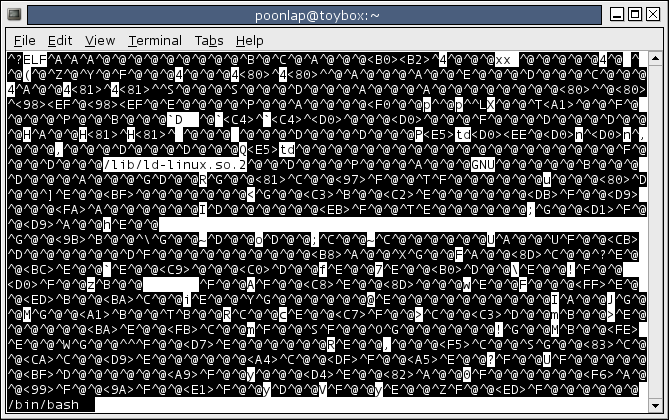
\includegraphics{less_binaryfile.eps}~~~~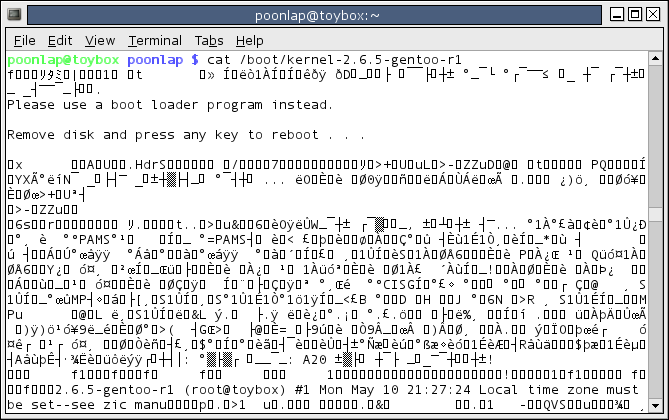
\includegraphics{cat_binaryfile.eps}}\caption{การดูไฟล์ไบนารีทางเทอร์มินอล}\label{fig:binfile}}}%
{\leftskip=\moveback\parbox{\headwidth}{\center\scalebox{.3}{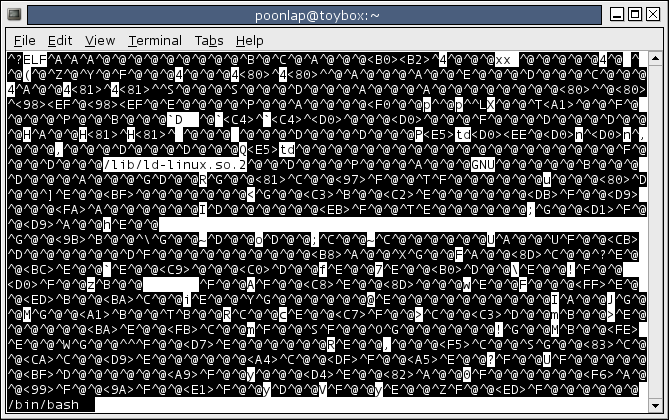
\includegraphics{less_binaryfile.eps}~~~~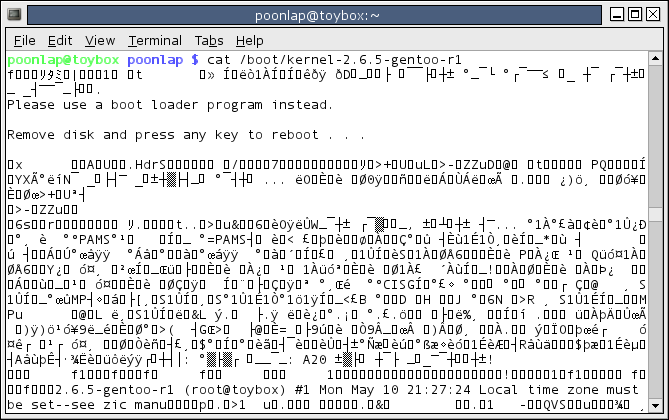
\includegraphics{cat_binaryfile.eps}}\caption{การดูไฟล์ไบนารีทางเทอร์มินอล}\label{fig:binfile}}}
\end{figure}
ในกรณีที่ใช้โปรแกรมที่ไม่มีการกรองอักขระควบคุมที่แสดงทางเทอร์มินอลเช่น \cmd{cat}, \cmd{head} ฯลฯ จะทำให้เทอร์มินอลแสดงผลหรือทำงานผิดปรกติหลังจากดูไฟล์ไบนารี. ในกรณีให้พิมพ์คำสั่ง \cmd{reset}\cindex{reset}\myexplanation{reset}{รีเซ็ตให้เทอร์มินอลอยู่ในสภาพเริ่มต้นปรกติ.} ถึงแม้จะอ่านไม่ออกก็ตามแล้วกดคีย์ \kk{Enter} ตาม. คำสั่ง \cmd{reset} จะทำให้เทอร์มินอลกลับอยู่ในสภาพปรกติ.

โอกาสที่จะดูเนื้อหาของไฟล์ไบนารีคงมีไม่บ่อยนักแต่ถ้ามีความจำเป็น, คำสั่ง \cmd{od}\cindex{od}\refcmd{od}\mymemo{ลินุกซ์ยังมีคำสั่งที่คล้ายกับคำสั่ง \cmd{od} อื่นๆอีกเช่น \cmd{hexdump}\cindex{hexdump}} %
ช่วยเราได้. 
\begin{MyExample}[ใช้ \cmd{od} ดูไฟล์ไบนารี.]
\begin{MyEx}
$ \cin{od /bin/bash | head -n 3}
0000000 042577 043114 000401 000001 000000 000000 000000 000000
0000020 000002 000003 000001 000000 131260 004005 000064 000000
0000040 074170 000011 000000 000000 000064 000040 000010 000050
\end{MyEx}
\end{MyExample}%$
ในแต่ละบรรทัดจะเป็นข้อมูลในไฟล์ที่แสดงในรูปของค่าฐานแปด. ถ้าต้องการให้แสดงข้อมูลเป็นฐานสิบหกให้ใช้ตัวเลือก \cmd{-h} (hexadecimal). อย่างไรก็ตามการข้อมูลที่แสดงนั้นไม่สื่อความหมายเท่าที่ควรเพราะเป็นตัวค่าของข้อมูลล้วนๆ. ถ้าใช้ตัวเลือก \cmd{-c} (character), คำสั่ง \cmd{od} จะพยายามแสดงข้อมูลที่เป็นอักขระ ASCII ทางหน้าจอ.
\begin{MyExample}[ใช้ \cmd{od} กับตัวเลือก \cmd{-c} ดูไฟล์ไบนารี.]\label{ex:od}
\begin{MyEx}
$ \cin{od -c /bin/bash | head -n 3}
0000000 177   E   L   F 001 001 001  \bs{}0  \bs{}0  \bs{}0  \bs{}0  \bs{}0  \bs{}0  \bs{}0  \bs{}0  \bs{}0
0000020 002  \bs{}0 003  \bs{}0 001  \bs{}0  \bs{}0  \bs{}0 260 262 005  \bs{}b   4  \bs{}0  \bs{}0  \bs{}0
0000040   x   x  \bs{}t  \bs{}0  \bs{}0  \bs{}0  \bs{}0  \bs{}0   4  \bs{}0      \bs{}0  \bs{}b  \bs{}0   (  \bs{}0
\end{MyEx}
\end{MyExample}%$
จะเห็นข้อมูลบางส่วนในไบนารีไฟล์มีข้อมูลเท็กซ์ผสมอยู่ด้วย. 

คำสั่ง \cmd{less}\refcmd{less} สามารถเปิดดูไฟล์ไบนารีได้เช่นเดียวกับการดูไฟล์เท็กซ์. จากรูปที่ \ref{fig:binfile} เป็นการใช้ \cmd{less} เปิดดูไฟล์ \cmd{/bin/bash} ซึ่งถ้าเปรียบเทียบกับตัวอย่างที่ \ref{ex:od} จะเห็นว่าคำสั่ง \cmd{less} จะแสดงส่วนที่เป็นอักขระ ASCII ให้. ถ้ามีการตั้งตัวแปรสภาพแวดล้อม \cmd{LESSOPEN} ไว้, \cmd{less} จะใช้โปรแกรมที่ระบุไว้ในตัวแปรนั้นเป็นโปรแกรมประมวลผลไฟล์ที่ต้องการดูข้อมูลก่อนที่จะใช้ \cmd{less} เปิดอ่านไฟล์นั้น. ตัวอย่างเช่นถ้าไฟล์ที่ต้องการเปิดอ่านด้วย \cmd{less} เป็นไฟล์ที่บีบอัดด้วย \cmd{gzip} (\cmd{.gz}), โปรแกรมที่ระบุไว้ในตัวแปรสภาพแวดล้อมก็จะใช้คำสั่ง \cmd{gzip} ขยายไฟล์นั้นก่อนแล้วส่งข้อมูลไปให้ \cmd{less}. ถ้าไม่ต้องการใช้โปรแกรมที่ระบุไว้ในตัวแปรสภาพแวดล้อม \cmd{LESSOPEN} ก็ใช้ใช้ตัวเลือก \cmd{-L}.

คำสั่งที่ใช้ดูข้อมูลเท็กซ์ที่อยู่ในไฟล์ไบนารีที่มีประโยชน์อีดคำสั่งคือ \cmd{strings}\cindex{strings}\refcmd{strings}. คำสั่ง \cmd{strings} จะสกัดส่วนที่เป็นข้อมูลเท็กซ์ออกมาจากไฟล์ไบนารี. ถ้าไม่มีการระบุตัวเลือก, คำสั่ง \cmd{strings} จะถือว่าข้อมูลเท็กซ์ที่ต้องการคืออักขระ ASCII ที่เรียงติดกันอย่างน้อย 4 ตัว. 
\begin{MyExample}[การสกัดส่วนที่เป็นข้อมูลเท็กซ์จากไฟล์ไบนารี.]
\begin{MyEx}
$ \cin{strings /bin/bash | head -n 3}
/lib/ld-linux.so.2
libdl.so.2
dlerror
\end{MyEx}
\end{MyExample}%$
สาเหตุที่คำสั่ง \cmd{strings} ไม่แสดงคำว่า ``ELF'' ทั้งๆที่คำสั่ง \cmd{od} เห็นว่ามีคำนี้เพราะว่าคำสั่ง \cmd{strings} จะสกัดข้อมูลเท็กซ์จากไฟล์ไบนารีที่เป็นไฟล์โปรแกรม, และจะสกัดข้อมูลเท็กซ์ที่อยู่ในช่วงของข้อมูลโปรแกรม (data sectoin) เท่านั้น. ถ้าต้องการจะให้คำสั่ง \cmd{strings} สกัดข้อมูลเท็กซ์จากทุกส่วนในไฟล์โปรแกรม, ให้ใช้ตัวเลือก \cmd{-a} (all) ประกอบ.
\begin{MyExample}[การใช้ \cmd{strings} กับตัวเลือก \cmd{-a}.]
\begin{MyEx}
$ \cin{strings -a -3 /bin/bash | head -n 3}
ELF
xx
`D
\end{MyEx}
\end{MyExample}%$



%\section{ไฟล์บราวเซอร์}
%สำหรับผู้ที่ยังไม่คุ้นเคยกับ

%gpathfinder, nautilus, konqueror, gtkfind


\section{สรุปท้ายบท}
\begin{itemize}
\item พาร์ทิชันคือการแบ่งฮาร์ดดิสก์เชิงตรรกะยังไม่สามารถใช้งานได้จนกว่าจะสร้างระบบไฟล์ในพาร์ทิชันนั้น.
\item ระบบไฟล์เชิงตรรกะในลินุกซ์จะมีโครงสร้างเป็นแผนภาพต้นไม้โดยมีไดเรกทอรีรูทเป็นจุดเริ่มต้นและขยายเป็นไดเรกทอรีย่อยต่อไป. 
\item การ mount คือการนำพาร์ทิชันมาปะติดกับไดเรกทอรีในระบบไฟล์.
\item ไฟล์คือกลุ่มข้อมูลหน่วยเป็นไบต์ที่เรียงเป็นลำดับต่อกันไปเป็นสาย.
\item ทุกอย่างในระบบปฏิบัติการยูนิกซ์และลินุกซ์สามารถแสดงได้ด้วยไฟล์.
\item ไดเรกทอรีคือไฟล์พิเศษที่มีข้อมูลเกี่ยวกับชื่อไฟล์และที่อยู่ในหน่วยความจำถาวรของไฟล์นั้น.
\item คำว่า ``ไฟล์'' มีความได้สองอย่างคือไฟล์จริง (ข้อมูล) หรือชื่อไฟล์ (ชื่ออ้างอิงข้อมูล).
%\item ในระบบปฏิบัติการลินุกซ์มีคำสั่งสำหรับจัดการ, ประมวลผลไฟล์หลายคำสั่ง. การศึกษาและใช้คำสั่งเหล่านี้ร่วมกันช่วยให้ผู้ใช้ทำงานได้คล่องและมีประสิทธิภาพ.
\end{itemize}
 
%\section{คำถามทบทวนความเข้าใจ}
%\begin{description}
%\myprac สมมติว่ามีไฟล์ชื่อ \cmd{-whatever}. จะลบไฟล์นี้ด้วยคำสั่ง \cmd{rm} ได้อย่างไร? (คำตอบหน้า \pageref{q_3_1})
%\myprac จงสังเกตตัวอย่างต่อไปนี้
%\begin{MyVerbatim}
%$ \cin{ls -l}
%total 0
%$ \cin{ls -al}
%total 8
%drwxr-xr-x    2 somchai  users        4096 May 30 18:21 ./
%-rw-r--r--    1 somchai  users           0 May 30 18:21 .
%-rw-r--r--    1 somchai  users           0 May 30 18:24 .
%drwx------   51 somchai  users        4096 May 30 17:40 ../
%$ \cin{rm .}
%rm: cannot remove `.' or `..'
%\end{MyVerbatim}
%จงให้เหตุผลที่เป็นไปได้ว่าทำไมมีไฟล์ ``\cmd{.}'' สองไฟล์. และจะลบเหล่านี้ได้อย่างไร? (\cmd{./} และ \cmd{../} คือไดเรกทอรี.) (คำตอบหน้า \pageref{q_3_2})
%\myprac ให้ไฟล์เสียง \cmd{.au} หรือ \cmd{.wav} ที่มีในระบบแล้วใช้ \cmd{cat} ฟังเสียงที่อยู่ในไฟล์นั้นๆ. (คำตอบหน้า \pageref{q_3_3})
%\myprac ให้ใช้คำสั่ง \cmd{cd} และ \cmd{ls} สำรวจโครงสร้างระบบไฟล์ไดเรกทอรีด้วยตัวเอง.
%\myprac ให้หาไฟล์ที่มีการตั้งค่าบิต suid และ sgid ที่อยู่ในไดเรกทอรี \cmd{/usr/bin}. (คำตอบหน้า \pageref{q_3_5})
%\myprac จงหาหลักฐาน (หรือข้อสันนิฐาน) ว่าเชลล์ \cmd{bash} พยายามอ่านไฟล์เริ่มต้นจาก \cmd{/etc/profile}, \cmd{~/.bash\_profile}. (คำตอบหน้า \pageref{q_3_6})
%\myprac ให้สำรวจว่าลินุกซ์ที่ผู้อ่านใช้อยู่มีการบันทึก atime ทุกครั้งที่ใช้ไฟล์หรือไม่. (คำตอบหน้า \pageref{q_3_7})
%\end{description}










\end{thwbr}
\wbrin